\documentclass[twoside]{book}

% Packages required by doxygen
\usepackage{fixltx2e}
\usepackage{calc}
\usepackage{doxygen}
\usepackage[export]{adjustbox} % also loads graphicx
\usepackage{graphicx}
\usepackage[utf8]{inputenc}
\usepackage{makeidx}
\usepackage{multicol}
\usepackage{multirow}
\PassOptionsToPackage{warn}{textcomp}
\usepackage{textcomp}
\usepackage[nointegrals]{wasysym}
\usepackage[table]{xcolor}

% Font selection
\usepackage[T1]{fontenc}
\usepackage[scaled=.90]{helvet}
\usepackage{courier}
\usepackage{amssymb}
\usepackage{sectsty}
\renewcommand{\familydefault}{\sfdefault}
\allsectionsfont{%
  \fontseries{bc}\selectfont%
  \color{darkgray}%
}
\renewcommand{\DoxyLabelFont}{%
  \fontseries{bc}\selectfont%
  \color{darkgray}%
}
\newcommand{\+}{\discretionary{\mbox{\scriptsize$\hookleftarrow$}}{}{}}

% Page & text layout
\usepackage{geometry}
\geometry{%
  a4paper,%
  top=2.5cm,%
  bottom=2.5cm,%
  left=2.5cm,%
  right=2.5cm%
}
\tolerance=750
\hfuzz=15pt
\hbadness=750
\setlength{\emergencystretch}{15pt}
\setlength{\parindent}{0cm}
\setlength{\parskip}{3ex plus 2ex minus 2ex}
\makeatletter
\renewcommand{\paragraph}{%
  \@startsection{paragraph}{4}{0ex}{-1.0ex}{1.0ex}{%
    \normalfont\normalsize\bfseries\SS@parafont%
  }%
}
\renewcommand{\subparagraph}{%
  \@startsection{subparagraph}{5}{0ex}{-1.0ex}{1.0ex}{%
    \normalfont\normalsize\bfseries\SS@subparafont%
  }%
}
\makeatother

% Headers & footers
\usepackage{fancyhdr}
\pagestyle{fancyplain}
\fancyhead[LE]{\fancyplain{}{\bfseries\thepage}}
\fancyhead[CE]{\fancyplain{}{}}
\fancyhead[RE]{\fancyplain{}{\bfseries\leftmark}}
\fancyhead[LO]{\fancyplain{}{\bfseries\rightmark}}
\fancyhead[CO]{\fancyplain{}{}}
\fancyhead[RO]{\fancyplain{}{\bfseries\thepage}}
\fancyfoot[LE]{\fancyplain{}{}}
\fancyfoot[CE]{\fancyplain{}{}}
\fancyfoot[RE]{\fancyplain{}{\bfseries\scriptsize Generated by Doxygen }}
\fancyfoot[LO]{\fancyplain{}{\bfseries\scriptsize Generated by Doxygen }}
\fancyfoot[CO]{\fancyplain{}{}}
\fancyfoot[RO]{\fancyplain{}{}}
\renewcommand{\footrulewidth}{0.4pt}
\renewcommand{\chaptermark}[1]{%
  \markboth{#1}{}%
}
\renewcommand{\sectionmark}[1]{%
  \markright{\thesection\ #1}%
}

% Indices & bibliography
\usepackage{natbib}
\usepackage[titles]{tocloft}
\setcounter{tocdepth}{3}
\setcounter{secnumdepth}{5}
\makeindex

% Hyperlinks (required, but should be loaded last)
\usepackage{ifpdf}
\ifpdf
  \usepackage[pdftex,pagebackref=true]{hyperref}
\else
  \usepackage[ps2pdf,pagebackref=true]{hyperref}
\fi
\hypersetup{%
  colorlinks=true,%
  linkcolor=blue,%
  citecolor=blue,%
  unicode%
}

% Custom commands
\newcommand{\clearemptydoublepage}{%
  \newpage{\pagestyle{empty}\cleardoublepage}%
}

\usepackage{caption}
\captionsetup{labelsep=space,justification=centering,font={bf},singlelinecheck=off,skip=4pt,position=top}

%===== C O N T E N T S =====

\begin{document}

% Titlepage & ToC
\hypersetup{pageanchor=false,
             bookmarksnumbered=true,
             pdfencoding=unicode
            }
\pagenumbering{alph}
\begin{titlepage}
\vspace*{7cm}
\begin{center}%
{\Large Deep Learning Based Object Detector \\[1ex]\large 1.\+0 }\\
\vspace*{1cm}
{\large Generated by Doxygen 1.8.14}\\
\end{center}
\end{titlepage}
\clearemptydoublepage
\pagenumbering{roman}
\tableofcontents
\clearemptydoublepage
\pagenumbering{arabic}
\hypersetup{pageanchor=true}

%--- Begin generated contents ---
\chapter{L\+I\+C\+E\+N\+SE}
\label{md__home_ravib_enpm808x-robotics-detection-module__l_i_c_e_n_s_e}
\Hypertarget{md__home_ravib_enpm808x-robotics-detection-module__l_i_c_e_n_s_e}
M\+IT License

Copyright (c) 2017 Ravi Bhadeshiya

Permission is hereby granted, free of charge, to any person obtaining a copy of this software and associated documentation files (the \char`\"{}\+Software\char`\"{}), to deal in the Software without restriction, including without limitation the rights to use, copy, modify, merge, publish, distribute, sublicense, and/or sell copies of the Software, and to permit persons to whom the Software is furnished to do so, subject to the following conditions\+:

The above copyright notice and this permission notice shall be included in all copies or substantial portions of the Software.

T\+HE S\+O\+F\+T\+W\+A\+RE IS P\+R\+O\+V\+I\+D\+ED \char`\"{}\+A\+S I\+S\char`\"{}, W\+I\+T\+H\+O\+UT W\+A\+R\+R\+A\+N\+TY OF A\+NY K\+I\+ND, E\+X\+P\+R\+E\+SS OR I\+M\+P\+L\+I\+ED, I\+N\+C\+L\+U\+D\+I\+NG B\+UT N\+OT L\+I\+M\+I\+T\+ED TO T\+HE W\+A\+R\+R\+A\+N\+T\+I\+ES OF M\+E\+R\+C\+H\+A\+N\+T\+A\+B\+I\+L\+I\+TY, F\+I\+T\+N\+E\+SS F\+OR A P\+A\+R\+T\+I\+C\+U\+L\+AR P\+U\+R\+P\+O\+SE A\+ND N\+O\+N\+I\+N\+F\+R\+I\+N\+G\+E\+M\+E\+NT. IN NO E\+V\+E\+NT S\+H\+A\+LL T\+HE A\+U\+T\+H\+O\+RS OR C\+O\+P\+Y\+R\+I\+G\+HT H\+O\+L\+D\+E\+RS BE L\+I\+A\+B\+LE F\+OR A\+NY C\+L\+A\+IM, D\+A\+M\+A\+G\+ES OR O\+T\+H\+ER L\+I\+A\+B\+I\+L\+I\+TY, W\+H\+E\+T\+H\+ER IN AN A\+C\+T\+I\+ON OF C\+O\+N\+T\+R\+A\+CT, T\+O\+RT OR O\+T\+H\+E\+R\+W\+I\+SE, A\+R\+I\+S\+I\+NG F\+R\+OM, O\+UT OF OR IN C\+O\+N\+N\+E\+C\+T\+I\+ON W\+I\+TH T\+HE S\+O\+F\+T\+W\+A\+RE OR T\+HE U\+SE OR O\+T\+H\+ER D\+E\+A\+L\+I\+N\+GS IN T\+HE S\+O\+F\+T\+W\+A\+RE. 
\chapter{Robotics detection modules}
\label{md__home_ravib_enpm808x-robotics-detection-module_readme}
\Hypertarget{md__home_ravib_enpm808x-robotics-detection-module_readme}
\href{https://travis-ci.org/raviBhadeshiya/enpm808x-robotics-detection-module}{\tt } \href{https://coveralls.io/github/raviBhadeshiya/enpm808x-robotics-detection-module?branch=master}{\tt } \hyperlink{_l_i_c_e_n_s_e_8md}{!\mbox{[}Packagist\mbox{]}(https\+://img.shields.io/packagist/l/doctrine/orm.svg)} 



\subsection*{Overview}

Midterm Project for E\+N\+P\+M808x\+: {\bfseries Deep Learning Based Object Detector}

Since the inception of the twenty-\/first century, the autonomous robot has been dominating the consumer market. To function properly in the unpredicted environment Re, they should avoid the collision, follow the lane properly and constantly look for a better path which requires knowledge of the environment. The robotics vision has made tremendous progress in addressing problems. In this midterm project, deep learning-\/based object detector implemented for A\+C\+ME Robotics which enable the robot to acquire knowledge of the environment and provide the ability to an appropriate reaction strategy or planning scheme; a simple and widely applicable strategy being to stop the robot.


\begin{DoxyItemize}
\item This detection module first preprocess input image and detect multiple object with help of \href{https://github.com/weiliu89/caffe/tree/ssd#models}{\tt pre-\/trained deep nerual net}. It will try to identify every object present in scenes and filter out some irrelevant objects with lower confidences which enable precision every time. The nerual net can be further trained for task relevant objects. The deep learning-\/based object detector can process approximately 30-\/25 F\+PS (depending on the speed of your system).
\item This module uses the technique called \href{https://arxiv.org/abs/1512.02325}{\tt Single-\/\+Shot Detector} to detect multiple objects on image. The Caffe based Open\+Cv Nerural Net was incorporated for this module. For more ref\+:\href{https://github.com/weiliu89/caffe/}{\tt Click Here}
\item For this module, \hyperlink{class_camera}{Camera} class was also developed to provide the input data for detection by reading jpg/png images or reading video files with format mp4/avi.\+However, with a little modification, it can access the any hardware cameara and provide the live stream for detection which is extremely useful for real-\/time.
\end{DoxyItemize}

\subsubsection*{Result}

The following result was shown by running the program with sample image sequences. Following sample images were processed with $\sim$40 ms time. 





 \subsubsection*{Required Depandencies}

\href{https://docs.opencv.org/trunk/d7/d9f/tutorial_linux_install.html}{\tt }

\#\#\# Build via command-\/line 
\begin{DoxyCode}
git clone --recursive https://github.com/raviBhadeshiya/enpm808x-robotics-detection-module.git
cd <path to repository>
mkdir build
cd build
cmake ..
make -j$(nproc)
\end{DoxyCode}

\begin{DoxyItemize}
\item To Run tests\+:{\ttfamily ./test/cpp-\/test}
\item To Run program\+:{\ttfamily ./app/shell-\/app $<$path$>$/filename}
\item To Run program with Image Sequence\+:{\ttfamily ./app/shell-\/app ../data/$\ast$.jpg}
\item To Run program with video\+:{\ttfamily ./app/shell-\/app ../data/test.mp4}
\end{DoxyItemize}

This detection module also support live stream from hardware camera which can be build by defining the preprocessor {\ttfamily \#define C\+A\+M\+E\+R\+A\+\_\+\+E\+N\+A\+B\+LE} in {\bfseries \hyperlink{_camera_8hpp}{Camera.\+hpp}} and following the build and running with {\ttfamily ./app/shell-\/app}. 

 \subsubsection*{Solo Iterative Process}

Solo Iterative process was used for developing this module It can be observed that estimates were improved over time. For detailed spreadsheet\+: \href{https://docs.google.com/spreadsheets/d/1QMfyDhY2k-3UoVmqBBLPma-o_mvVv3tEnGuCV8GbJtA/edit?usp=sharing}{\tt } 

 
\chapter{Hierarchical Index}
\section{Class Hierarchy}
This inheritance list is sorted roughly, but not completely, alphabetically\+:\begin{DoxyCompactList}
\item \contentsline{section}{Module}{\pageref{class_module}}{}
\begin{DoxyCompactList}
\item \contentsline{section}{Detection}{\pageref{class_detection}}{}
\end{DoxyCompactList}
\item \contentsline{section}{Robot}{\pageref{class_robot}}{}
\item \contentsline{section}{Sensor$<$ T $>$}{\pageref{class_sensor}}{}
\item \contentsline{section}{Sensor$<$ cv\+:\+:Mat $>$}{\pageref{class_sensor}}{}
\begin{DoxyCompactList}
\item \contentsline{section}{Camera}{\pageref{class_camera}}{}
\end{DoxyCompactList}
\end{DoxyCompactList}

\chapter{Class Index}
\section{Class List}
Here are the classes, structs, unions and interfaces with brief descriptions\+:\begin{DoxyCompactList}
\item\contentsline{section}{\hyperlink{class_camera}{Camera} \\*Class for camera inherited from sensor }{\pageref{class_camera}}{}
\item\contentsline{section}{\hyperlink{class_detection}{Detection} \\*Class for object detection }{\pageref{class_detection}}{}
\item\contentsline{section}{\hyperlink{class_module}{Module} \\*Virtual Class for detection module }{\pageref{class_module}}{}
\item\contentsline{section}{\hyperlink{class_robot}{Robot} \\*Class for robot }{\pageref{class_robot}}{}
\item\contentsline{section}{\hyperlink{class_sensor}{Sensor$<$ T $>$} \\*Virtual Class for every sensor }{\pageref{class_sensor}}{}
\end{DoxyCompactList}

\chapter{File Index}
\section{File List}
Here is a list of all files with brief descriptions\+:\begin{DoxyCompactList}
\item\contentsline{section}{/home/ravib/enpm808x-\/robotics-\/detection-\/module/\hyperlink{_8ycm__extra__conf_8py}{.\+ycm\+\_\+extra\+\_\+conf.\+py} }{\pageref{_8ycm__extra__conf_8py}}{}
\item\contentsline{section}{/home/ravib/enpm808x-\/robotics-\/detection-\/module/app/\hyperlink{_camera_8cpp}{Camera.\+cpp} }{\pageref{_camera_8cpp}}{}
\item\contentsline{section}{/home/ravib/enpm808x-\/robotics-\/detection-\/module/app/\hyperlink{_detection_8cpp}{Detection.\+cpp} }{\pageref{_detection_8cpp}}{}
\item\contentsline{section}{/home/ravib/enpm808x-\/robotics-\/detection-\/module/app/\hyperlink{app_2main_8cpp}{main.\+cpp} }{\pageref{app_2main_8cpp}}{}
\item\contentsline{section}{/home/ravib/enpm808x-\/robotics-\/detection-\/module/app/\hyperlink{_robot_8cpp}{Robot.\+cpp} }{\pageref{_robot_8cpp}}{}
\item\contentsline{section}{/home/ravib/enpm808x-\/robotics-\/detection-\/module/build/\+C\+Make\+Files/\hyperlink{feature__tests_8c}{feature\+\_\+tests.\+c} }{\pageref{feature__tests_8c}}{}
\item\contentsline{section}{/home/ravib/enpm808x-\/robotics-\/detection-\/module/build/\+C\+Make\+Files/\hyperlink{feature__tests_8cxx}{feature\+\_\+tests.\+cxx} }{\pageref{feature__tests_8cxx}}{}
\item\contentsline{section}{/home/ravib/enpm808x-\/robotics-\/detection-\/module/build/\+C\+Make\+Files/3.\+5.\+1/\+Compiler\+Id\+C/\hyperlink{_c_make_c_compiler_id_8c}{C\+Make\+C\+Compiler\+Id.\+c} }{\pageref{_c_make_c_compiler_id_8c}}{}
\item\contentsline{section}{/home/ravib/enpm808x-\/robotics-\/detection-\/module/build/\+C\+Make\+Files/3.\+5.\+1/\+Compiler\+Id\+C\+X\+X/\hyperlink{_c_make_c_x_x_compiler_id_8cpp}{C\+Make\+C\+X\+X\+Compiler\+Id.\+cpp} }{\pageref{_c_make_c_x_x_compiler_id_8cpp}}{}
\item\contentsline{section}{/home/ravib/enpm808x-\/robotics-\/detection-\/module/include/\hyperlink{_camera_8hpp}{Camera.\+hpp} \\*Robotics\+\_\+detection\+\_\+module }{\pageref{_camera_8hpp}}{}
\item\contentsline{section}{/home/ravib/enpm808x-\/robotics-\/detection-\/module/include/\hyperlink{_detection_8hpp}{Detection.\+hpp} \\*Deep Nerual Net based \hyperlink{class_detection}{Detection} \hyperlink{class_module}{Module} }{\pageref{_detection_8hpp}}{}
\item\contentsline{section}{/home/ravib/enpm808x-\/robotics-\/detection-\/module/include/\hyperlink{_module_8hpp}{Module.\+hpp} }{\pageref{_module_8hpp}}{}
\item\contentsline{section}{/home/ravib/enpm808x-\/robotics-\/detection-\/module/include/\hyperlink{_robot_8hpp}{Robot.\+hpp} \\*\hyperlink{class_robot}{Robot} module for handling everthing }{\pageref{_robot_8hpp}}{}
\item\contentsline{section}{/home/ravib/enpm808x-\/robotics-\/detection-\/module/include/\hyperlink{_sensor_8hpp}{Sensor.\+hpp} }{\pageref{_sensor_8hpp}}{}
\item\contentsline{section}{/home/ravib/enpm808x-\/robotics-\/detection-\/module/test/\hyperlink{test_2main_8cpp}{main.\+cpp} }{\pageref{test_2main_8cpp}}{}
\item\contentsline{section}{/home/ravib/enpm808x-\/robotics-\/detection-\/module/test/\hyperlink{_mock_camera_8cpp}{Mock\+Camera.\+cpp} }{\pageref{_mock_camera_8cpp}}{}
\item\contentsline{section}{/home/ravib/enpm808x-\/robotics-\/detection-\/module/test/\hyperlink{_mock_detection_8cpp}{Mock\+Detection.\+cpp} }{\pageref{_mock_detection_8cpp}}{}
\item\contentsline{section}{/home/ravib/enpm808x-\/robotics-\/detection-\/module/test/\hyperlink{_mock_robot_8cpp}{Mock\+Robot.\+cpp} }{\pageref{_mock_robot_8cpp}}{}
\end{DoxyCompactList}

\chapter{Class Documentation}
\hypertarget{class_camera}{}\section{Camera Class Reference}
\label{class_camera}\index{Camera@{Camera}}


Class for camera inherited from sensor.  




{\ttfamily \#include $<$Camera.\+hpp$>$}



Inheritance diagram for Camera\+:
\nopagebreak
\begin{figure}[H]
\begin{center}
\leavevmode
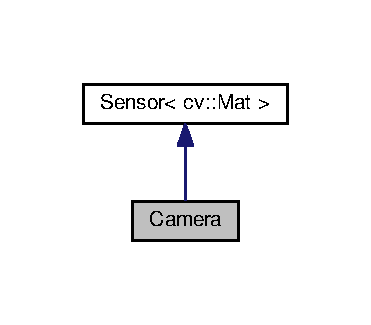
\includegraphics[width=178pt]{class_camera__inherit__graph}
\end{center}
\end{figure}


Collaboration diagram for Camera\+:
\nopagebreak
\begin{figure}[H]
\begin{center}
\leavevmode
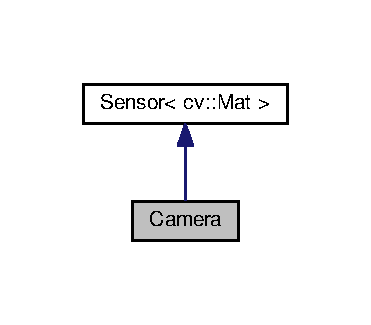
\includegraphics[width=178pt]{class_camera__coll__graph}
\end{center}
\end{figure}
\subsection*{Public Member Functions}
\begin{DoxyCompactItemize}
\item 
\hyperlink{class_camera_a01f94c3543f56ede7af49dc778f19331}{Camera} ()
\begin{DoxyCompactList}\small\item\em Create the camera object. \end{DoxyCompactList}\item 
\hyperlink{class_camera_ae105913661d2f33f91bdfb5a6ab1db8b}{Camera} (const std\+::string \&file)
\begin{DoxyCompactList}\small\item\em Create specific the camera object as per file name. \end{DoxyCompactList}\item 
\hyperlink{class_camera_a06c600e443fd9222c1fd4c13b9bdfd09}{Camera} (const int \&device\+Id)
\begin{DoxyCompactList}\small\item\em Create camera object to access the hardware. \end{DoxyCompactList}\item 
\hyperlink{class_camera_ad1897942d0ccf91052386388a497349f}{$\sim$\+Camera} ()
\begin{DoxyCompactList}\small\item\em Destroys the object. \end{DoxyCompactList}\item 
auto \hyperlink{class_camera_ae957cc994193c4a367d1e592a16a477f}{update} () -\/$>$ void
\begin{DoxyCompactList}\small\item\em Update method. \end{DoxyCompactList}\item 
auto \hyperlink{class_camera_a635f36e95291ad8962a6b85bf2a12def}{is\+Opened} () -\/$>$ bool
\begin{DoxyCompactList}\small\item\em Determines if \hyperlink{class_camera}{Camera} running. \end{DoxyCompactList}\item 
auto \hyperlink{class_camera_a4e83407793c8388903a37e29925e4bb5}{is\+Image\+Seq} () -\/$>$ bool
\begin{DoxyCompactList}\small\item\em Determines if image sequence. \end{DoxyCompactList}\item 
auto \hyperlink{class_camera_acd484ba9de5bb9f6a86bf40396dc4e69}{get\+Data} () -\/$>$ cv\+::\+Mat
\begin{DoxyCompactList}\small\item\em Gets the data. \end{DoxyCompactList}\item 
auto \hyperlink{class_camera_a6d379d7a64c1469edad924b925cdcb1d}{get\+Filenames} () -\/$>$ std\+::vector$<$ cv\+::\+String $>$
\begin{DoxyCompactList}\small\item\em Gets the filenames. \end{DoxyCompactList}\end{DoxyCompactItemize}


\subsection{Detailed Description}
Class for camera inherited from sensor. 

Definition at line 27 of file Camera.\+hpp.



\subsection{Constructor \& Destructor Documentation}
\mbox{\Hypertarget{class_camera_a01f94c3543f56ede7af49dc778f19331}\label{class_camera_a01f94c3543f56ede7af49dc778f19331}} 
\index{Camera@{Camera}!Camera@{Camera}}
\index{Camera@{Camera}!Camera@{Camera}}
\subsubsection{\texorpdfstring{Camera()}{Camera()}\hspace{0.1cm}{\footnotesize\ttfamily [1/3]}}
{\footnotesize\ttfamily Camera\+::\+Camera (\begin{DoxyParamCaption}{ }\end{DoxyParamCaption})}



Create the camera object. 



Definition at line 12 of file Camera.\+cpp.

\mbox{\Hypertarget{class_camera_ae105913661d2f33f91bdfb5a6ab1db8b}\label{class_camera_ae105913661d2f33f91bdfb5a6ab1db8b}} 
\index{Camera@{Camera}!Camera@{Camera}}
\index{Camera@{Camera}!Camera@{Camera}}
\subsubsection{\texorpdfstring{Camera()}{Camera()}\hspace{0.1cm}{\footnotesize\ttfamily [2/3]}}
{\footnotesize\ttfamily Camera\+::\+Camera (\begin{DoxyParamCaption}\item[{const std\+::string \&}]{file }\end{DoxyParamCaption})\hspace{0.3cm}{\ttfamily [explicit]}}



Create specific the camera object as per file name. 


\begin{DoxyParams}[1]{Parameters}
\mbox{\tt in}  & {\em id} & The device identifier. \\
\hline
\end{DoxyParams}


Definition at line 15 of file Camera.\+cpp.

\mbox{\Hypertarget{class_camera_a06c600e443fd9222c1fd4c13b9bdfd09}\label{class_camera_a06c600e443fd9222c1fd4c13b9bdfd09}} 
\index{Camera@{Camera}!Camera@{Camera}}
\index{Camera@{Camera}!Camera@{Camera}}
\subsubsection{\texorpdfstring{Camera()}{Camera()}\hspace{0.1cm}{\footnotesize\ttfamily [3/3]}}
{\footnotesize\ttfamily Camera\+::\+Camera (\begin{DoxyParamCaption}\item[{const int \&}]{device\+Id }\end{DoxyParamCaption})\hspace{0.3cm}{\ttfamily [explicit]}}



Create camera object to access the hardware. 


\begin{DoxyParams}[1]{Parameters}
\mbox{\tt in}  & {\em device\+Id} & The hardware device identifier \\
\hline
\end{DoxyParams}
\mbox{\Hypertarget{class_camera_ad1897942d0ccf91052386388a497349f}\label{class_camera_ad1897942d0ccf91052386388a497349f}} 
\index{Camera@{Camera}!````~Camera@{$\sim$\+Camera}}
\index{````~Camera@{$\sim$\+Camera}!Camera@{Camera}}
\subsubsection{\texorpdfstring{$\sim$\+Camera()}{~Camera()}}
{\footnotesize\ttfamily Camera\+::$\sim$\+Camera (\begin{DoxyParamCaption}{ }\end{DoxyParamCaption})}



Destroys the object. 



Definition at line 56 of file Camera.\+cpp.



\subsection{Member Function Documentation}
\mbox{\Hypertarget{class_camera_acd484ba9de5bb9f6a86bf40396dc4e69}\label{class_camera_acd484ba9de5bb9f6a86bf40396dc4e69}} 
\index{Camera@{Camera}!get\+Data@{get\+Data}}
\index{get\+Data@{get\+Data}!Camera@{Camera}}
\subsubsection{\texorpdfstring{get\+Data()}{getData()}}
{\footnotesize\ttfamily auto Camera\+::get\+Data (\begin{DoxyParamCaption}{ }\end{DoxyParamCaption}) -\/$>$ cv\+::\+Mat\hspace{0.3cm}{\ttfamily [virtual]}}



Gets the data. 

\begin{DoxyReturn}{Returns}
The data. 
\end{DoxyReturn}


Implements \hyperlink{class_sensor_ae9ab3f3715367df03900706eb9806afd}{Sensor$<$ cv\+::\+Mat $>$}.



Definition at line 77 of file Camera.\+cpp.

\mbox{\Hypertarget{class_camera_a6d379d7a64c1469edad924b925cdcb1d}\label{class_camera_a6d379d7a64c1469edad924b925cdcb1d}} 
\index{Camera@{Camera}!get\+Filenames@{get\+Filenames}}
\index{get\+Filenames@{get\+Filenames}!Camera@{Camera}}
\subsubsection{\texorpdfstring{get\+Filenames()}{getFilenames()}}
{\footnotesize\ttfamily auto Camera\+::get\+Filenames (\begin{DoxyParamCaption}{ }\end{DoxyParamCaption}) -\/$>$ std\+::vector$<$cv\+::\+String$>$}



Gets the filenames. 

\begin{DoxyReturn}{Returns}
The filenames. 
\end{DoxyReturn}


Definition at line 89 of file Camera.\+cpp.

\mbox{\Hypertarget{class_camera_a4e83407793c8388903a37e29925e4bb5}\label{class_camera_a4e83407793c8388903a37e29925e4bb5}} 
\index{Camera@{Camera}!is\+Image\+Seq@{is\+Image\+Seq}}
\index{is\+Image\+Seq@{is\+Image\+Seq}!Camera@{Camera}}
\subsubsection{\texorpdfstring{is\+Image\+Seq()}{isImageSeq()}}
{\footnotesize\ttfamily auto Camera\+::is\+Image\+Seq (\begin{DoxyParamCaption}{ }\end{DoxyParamCaption}) -\/$>$ bool}



Determines if image sequence. 

\begin{DoxyReturn}{Returns}
True if image sequence, False otherwise. 
\end{DoxyReturn}


Definition at line 94 of file Camera.\+cpp.

\mbox{\Hypertarget{class_camera_a635f36e95291ad8962a6b85bf2a12def}\label{class_camera_a635f36e95291ad8962a6b85bf2a12def}} 
\index{Camera@{Camera}!is\+Opened@{is\+Opened}}
\index{is\+Opened@{is\+Opened}!Camera@{Camera}}
\subsubsection{\texorpdfstring{is\+Opened()}{isOpened()}}
{\footnotesize\ttfamily auto Camera\+::is\+Opened (\begin{DoxyParamCaption}{ }\end{DoxyParamCaption}) -\/$>$ bool\hspace{0.3cm}{\ttfamily [virtual]}}



Determines if \hyperlink{class_camera}{Camera} running. 

\begin{DoxyReturn}{Returns}
True if \hyperlink{class_camera}{Camera} running, False otherwise. 
\end{DoxyReturn}


Implements \hyperlink{class_sensor_a78f10e5c1fd3c7e5fcbbf4ca735ac1e7}{Sensor$<$ cv\+::\+Mat $>$}.



Definition at line 83 of file Camera.\+cpp.

\mbox{\Hypertarget{class_camera_ae957cc994193c4a367d1e592a16a477f}\label{class_camera_ae957cc994193c4a367d1e592a16a477f}} 
\index{Camera@{Camera}!update@{update}}
\index{update@{update}!Camera@{Camera}}
\subsubsection{\texorpdfstring{update()}{update()}}
{\footnotesize\ttfamily auto Camera\+::update (\begin{DoxyParamCaption}{ }\end{DoxyParamCaption}) -\/$>$ void\hspace{0.3cm}{\ttfamily [virtual]}}



Update method. 

\begin{DoxyReturn}{Returns}
return none. 
\end{DoxyReturn}


Implements \hyperlink{class_sensor_a1766329f3c9918fa886ead46b141a6a8}{Sensor$<$ cv\+::\+Mat $>$}.



Definition at line 59 of file Camera.\+cpp.



The documentation for this class was generated from the following files\+:\begin{DoxyCompactItemize}
\item 
/home/ravib/enpm808x-\/robotics-\/detection-\/module/include/\hyperlink{_camera_8hpp}{Camera.\+hpp}\item 
/home/ravib/enpm808x-\/robotics-\/detection-\/module/app/\hyperlink{_camera_8cpp}{Camera.\+cpp}\end{DoxyCompactItemize}

\hypertarget{class_detection}{}\section{Detection Class Reference}
\label{class_detection}\index{Detection@{Detection}}


Class for object detection.  




{\ttfamily \#include $<$Detection.\+hpp$>$}



Inheritance diagram for Detection\+:
\nopagebreak
\begin{figure}[H]
\begin{center}
\leavevmode
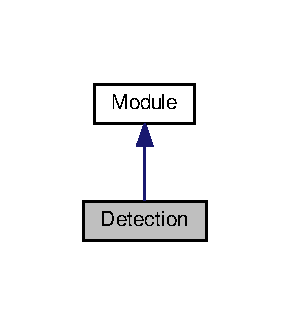
\includegraphics[width=139pt]{class_detection__inherit__graph}
\end{center}
\end{figure}


Collaboration diagram for Detection\+:
\nopagebreak
\begin{figure}[H]
\begin{center}
\leavevmode
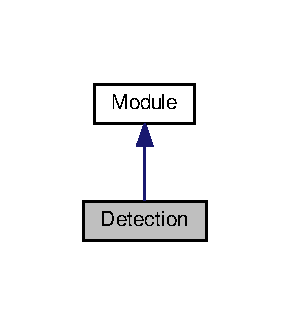
\includegraphics[width=139pt]{class_detection__coll__graph}
\end{center}
\end{figure}
\subsection*{Public Member Functions}
\begin{DoxyCompactItemize}
\item 
\hyperlink{class_detection_a86e6ebf5a660a29e78ee7a7f08292260}{Detection} ()
\begin{DoxyCompactList}\small\item\em Create a detector. \end{DoxyCompactList}\item 
\hyperlink{class_detection_a27315b70fad96e80db6a5b9f52fe7071}{Detection} (const cv\+::\+String \&model\+Config, const cv\+::\+String \&binary)
\begin{DoxyCompactList}\small\item\em Overloaded constructor for defining parameter. \end{DoxyCompactList}\item 
\hyperlink{class_detection_abbfdeb60a10132d820fcd20dd292e400}{$\sim$\+Detection} ()
\begin{DoxyCompactList}\small\item\em Destroys the detector. \end{DoxyCompactList}\item 
auto \hyperlink{class_detection_a7ec75616ce302825816a0ee350452ef8}{update} (const cv\+::\+Mat \&frame) -\/$>$ cv\+::\+Mat
\begin{DoxyCompactList}\small\item\em Update method for updating every thing. \end{DoxyCompactList}\item 
auto \hyperlink{class_detection_a5a959a3e87c5cfba1ae5a78429df6b5c}{update} () -\/$>$ void
\begin{DoxyCompactList}\small\item\em Overloaded Update method for updating every thing for internal image. \end{DoxyCompactList}\item 
auto \hyperlink{class_detection_aa1bbf9f6725e8f412f694ca7cf759ff5}{get\+Objects} (const cv\+::\+Mat \&frame) -\/$>$ cv\+::\+Mat
\begin{DoxyCompactList}\small\item\em Gets the objects. \end{DoxyCompactList}\item 
auto \hyperlink{class_detection_a898f16ebdea8c1c3cc2cd789a9bfadc9}{pre\+Process} (const cv\+::\+Mat \&frame) -\/$>$ cv\+::\+Mat
\begin{DoxyCompactList}\small\item\em Preprocess the image for clear detection. \end{DoxyCompactList}\item 
auto \hyperlink{class_detection_a1a481a0248acb74cb0df6bcd437783eb}{render} (cv\+::\+Mat frame, const cv\+::\+Mat \&detection\+Mat) -\/$>$ cv\+::\+Mat
\begin{DoxyCompactList}\small\item\em Render the bounding box over the object. \end{DoxyCompactList}\item 
auto \hyperlink{class_detection_a3a657b6943cacfd4bdd55d90def58427}{is\+Setup} (void) -\/$>$ bool
\begin{DoxyCompactList}\small\item\em Determines if setup. \end{DoxyCompactList}\item 
auto \hyperlink{class_detection_a3340560fb1e76bd096478d4c29306130}{get\+Mean} (const int \&width, const int \&height) -\/$>$ cv\+::\+Mat
\begin{DoxyCompactList}\small\item\em Gets the mean. \end{DoxyCompactList}\item 
auto \hyperlink{class_detection_a0f4577baa1334c17054489a3ab8804ba}{import} () -\/$>$ void
\begin{DoxyCompactList}\small\item\em Refactored function for importing. \end{DoxyCompactList}\end{DoxyCompactItemize}


\subsection{Detailed Description}
Class for object detection. 

Definition at line 37 of file Detection.\+hpp.



\subsection{Constructor \& Destructor Documentation}
\mbox{\Hypertarget{class_detection_a86e6ebf5a660a29e78ee7a7f08292260}\label{class_detection_a86e6ebf5a660a29e78ee7a7f08292260}} 
\index{Detection@{Detection}!Detection@{Detection}}
\index{Detection@{Detection}!Detection@{Detection}}
\subsubsection{\texorpdfstring{Detection()}{Detection()}\hspace{0.1cm}{\footnotesize\ttfamily [1/2]}}
{\footnotesize\ttfamily Detection\+::\+Detection (\begin{DoxyParamCaption}{ }\end{DoxyParamCaption})}



Create a detector. 



Definition at line 11 of file Detection.\+cpp.

\mbox{\Hypertarget{class_detection_a27315b70fad96e80db6a5b9f52fe7071}\label{class_detection_a27315b70fad96e80db6a5b9f52fe7071}} 
\index{Detection@{Detection}!Detection@{Detection}}
\index{Detection@{Detection}!Detection@{Detection}}
\subsubsection{\texorpdfstring{Detection()}{Detection()}\hspace{0.1cm}{\footnotesize\ttfamily [2/2]}}
{\footnotesize\ttfamily Detection\+::\+Detection (\begin{DoxyParamCaption}\item[{const cv\+::\+String \&}]{model\+Config,  }\item[{const cv\+::\+String \&}]{binary }\end{DoxyParamCaption})}



Overloaded constructor for defining parameter. 


\begin{DoxyParams}[1]{Parameters}
\mbox{\tt in}  & {\em model\+Config} & The model configuration \\
\hline
\mbox{\tt in}  & {\em binary} & The binary \\
\hline
\mbox{\tt in}  & {\em import\+Also} & The import also \\
\hline
\end{DoxyParams}


Definition at line 13 of file Detection.\+cpp.

\mbox{\Hypertarget{class_detection_abbfdeb60a10132d820fcd20dd292e400}\label{class_detection_abbfdeb60a10132d820fcd20dd292e400}} 
\index{Detection@{Detection}!````~Detection@{$\sim$\+Detection}}
\index{````~Detection@{$\sim$\+Detection}!Detection@{Detection}}
\subsubsection{\texorpdfstring{$\sim$\+Detection()}{~Detection()}}
{\footnotesize\ttfamily Detection\+::$\sim$\+Detection (\begin{DoxyParamCaption}{ }\end{DoxyParamCaption})}



Destroys the detector. 



Definition at line 21 of file Detection.\+cpp.



\subsection{Member Function Documentation}
\mbox{\Hypertarget{class_detection_a3340560fb1e76bd096478d4c29306130}\label{class_detection_a3340560fb1e76bd096478d4c29306130}} 
\index{Detection@{Detection}!get\+Mean@{get\+Mean}}
\index{get\+Mean@{get\+Mean}!Detection@{Detection}}
\subsubsection{\texorpdfstring{get\+Mean()}{getMean()}}
{\footnotesize\ttfamily auto Detection\+::get\+Mean (\begin{DoxyParamCaption}\item[{const int \&}]{width,  }\item[{const int \&}]{height }\end{DoxyParamCaption}) -\/$>$ cv\+::\+Mat}



Gets the mean. 


\begin{DoxyParams}[1]{Parameters}
\mbox{\tt in}  & {\em width} & The width \\
\hline
\mbox{\tt in}  & {\em height} & The height\\
\hline
\end{DoxyParams}
\begin{DoxyReturn}{Returns}
The mean as image 
\end{DoxyReturn}


Definition at line 89 of file Detection.\+cpp.

\mbox{\Hypertarget{class_detection_aa1bbf9f6725e8f412f694ca7cf759ff5}\label{class_detection_aa1bbf9f6725e8f412f694ca7cf759ff5}} 
\index{Detection@{Detection}!get\+Objects@{get\+Objects}}
\index{get\+Objects@{get\+Objects}!Detection@{Detection}}
\subsubsection{\texorpdfstring{get\+Objects()}{getObjects()}}
{\footnotesize\ttfamily auto Detection\+::get\+Objects (\begin{DoxyParamCaption}\item[{const cv\+::\+Mat \&}]{frame }\end{DoxyParamCaption}) -\/$>$ cv\+::\+Mat}



Gets the objects. 


\begin{DoxyParams}[1]{Parameters}
\mbox{\tt in}  & {\em frame} & Input frame as image\\
\hline
\end{DoxyParams}
\begin{DoxyReturn}{Returns}
return the detected object as image 
\end{DoxyReturn}


Definition at line 57 of file Detection.\+cpp.

\mbox{\Hypertarget{class_detection_a0f4577baa1334c17054489a3ab8804ba}\label{class_detection_a0f4577baa1334c17054489a3ab8804ba}} 
\index{Detection@{Detection}!import@{import}}
\index{import@{import}!Detection@{Detection}}
\subsubsection{\texorpdfstring{import()}{import()}}
{\footnotesize\ttfamily auto Detection\+::import (\begin{DoxyParamCaption}{ }\end{DoxyParamCaption}) -\/$>$ void}



Refactored function for importing. 

\begin{DoxyReturn}{Returns}
Return none 
\end{DoxyReturn}


Definition at line 23 of file Detection.\+cpp.

\mbox{\Hypertarget{class_detection_a3a657b6943cacfd4bdd55d90def58427}\label{class_detection_a3a657b6943cacfd4bdd55d90def58427}} 
\index{Detection@{Detection}!is\+Setup@{is\+Setup}}
\index{is\+Setup@{is\+Setup}!Detection@{Detection}}
\subsubsection{\texorpdfstring{is\+Setup()}{isSetup()}}
{\footnotesize\ttfamily auto Detection\+::is\+Setup (\begin{DoxyParamCaption}\item[{void}]{ }\end{DoxyParamCaption}) -\/$>$ bool\hspace{0.3cm}{\ttfamily [virtual]}}



Determines if setup. 

\begin{DoxyReturn}{Returns}
True if setup, False otherwise 
\end{DoxyReturn}


Implements \hyperlink{class_module_a20fb30b0bf6ea415e93efbbacc68043c}{Module}.



Definition at line 155 of file Detection.\+cpp.

\mbox{\Hypertarget{class_detection_a898f16ebdea8c1c3cc2cd789a9bfadc9}\label{class_detection_a898f16ebdea8c1c3cc2cd789a9bfadc9}} 
\index{Detection@{Detection}!pre\+Process@{pre\+Process}}
\index{pre\+Process@{pre\+Process}!Detection@{Detection}}
\subsubsection{\texorpdfstring{pre\+Process()}{preProcess()}}
{\footnotesize\ttfamily auto Detection\+::pre\+Process (\begin{DoxyParamCaption}\item[{const cv\+::\+Mat \&}]{frame }\end{DoxyParamCaption}) -\/$>$ cv\+::\+Mat}



Preprocess the image for clear detection. 


\begin{DoxyParams}[1]{Parameters}
\mbox{\tt in}  & {\em frame} & Input frame as image\\
\hline
\end{DoxyParams}
\begin{DoxyReturn}{Returns}
return the processed image as image 
\end{DoxyReturn}


Definition at line 74 of file Detection.\+cpp.

\mbox{\Hypertarget{class_detection_a1a481a0248acb74cb0df6bcd437783eb}\label{class_detection_a1a481a0248acb74cb0df6bcd437783eb}} 
\index{Detection@{Detection}!render@{render}}
\index{render@{render}!Detection@{Detection}}
\subsubsection{\texorpdfstring{render()}{render()}}
{\footnotesize\ttfamily auto Detection\+::render (\begin{DoxyParamCaption}\item[{cv\+::\+Mat}]{frame,  }\item[{const cv\+::\+Mat \&}]{detection\+Mat }\end{DoxyParamCaption}) -\/$>$ cv\+::\+Mat}



Render the bounding box over the object. 


\begin{DoxyParams}[1]{Parameters}
\mbox{\tt in}  & {\em frame} & Input frame as image\\
\hline
\end{DoxyParams}
\begin{DoxyReturn}{Returns}
return the rendered object as image 
\end{DoxyReturn}


Definition at line 103 of file Detection.\+cpp.

\mbox{\Hypertarget{class_detection_a7ec75616ce302825816a0ee350452ef8}\label{class_detection_a7ec75616ce302825816a0ee350452ef8}} 
\index{Detection@{Detection}!update@{update}}
\index{update@{update}!Detection@{Detection}}
\subsubsection{\texorpdfstring{update()}{update()}\hspace{0.1cm}{\footnotesize\ttfamily [1/2]}}
{\footnotesize\ttfamily auto Detection\+::update (\begin{DoxyParamCaption}\item[{const cv\+::\+Mat \&}]{frame }\end{DoxyParamCaption}) -\/$>$ cv\+::\+Mat}



Update method for updating every thing. 


\begin{DoxyParams}[1]{Parameters}
\mbox{\tt in}  & {\em frame} & The frame as image\\
\hline
\end{DoxyParams}
\begin{DoxyReturn}{Returns}
return image with detected content if any 
\end{DoxyReturn}


Definition at line 41 of file Detection.\+cpp.

\mbox{\Hypertarget{class_detection_a5a959a3e87c5cfba1ae5a78429df6b5c}\label{class_detection_a5a959a3e87c5cfba1ae5a78429df6b5c}} 
\index{Detection@{Detection}!update@{update}}
\index{update@{update}!Detection@{Detection}}
\subsubsection{\texorpdfstring{update()}{update()}\hspace{0.1cm}{\footnotesize\ttfamily [2/2]}}
{\footnotesize\ttfamily auto Detection\+::update (\begin{DoxyParamCaption}\item[{void}]{ }\end{DoxyParamCaption}) -\/$>$ void\hspace{0.3cm}{\ttfamily [virtual]}}



Overloaded Update method for updating every thing for internal image. 

\begin{DoxyReturn}{Returns}
return image with detected content if any 
\end{DoxyReturn}


Implements \hyperlink{class_module_a21af40d45926cf90d6573f5ac5a1149f}{Module}.



Definition at line 52 of file Detection.\+cpp.



The documentation for this class was generated from the following files\+:\begin{DoxyCompactItemize}
\item 
/home/ravib/enpm808x-\/robotics-\/detection-\/module/include/\hyperlink{_detection_8hpp}{Detection.\+hpp}\item 
/home/ravib/enpm808x-\/robotics-\/detection-\/module/app/\hyperlink{_detection_8cpp}{Detection.\+cpp}\end{DoxyCompactItemize}

\hypertarget{class_module}{}\section{Module Class Reference}
\label{class_module}\index{Module@{Module}}


Virtual Class for detection module.  




{\ttfamily \#include $<$Module.\+hpp$>$}



Inheritance diagram for Module\+:
\nopagebreak
\begin{figure}[H]
\begin{center}
\leavevmode
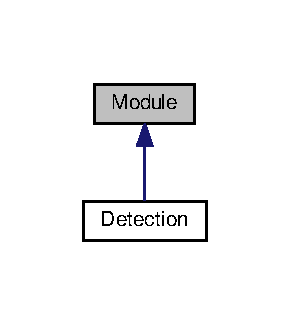
\includegraphics[width=139pt]{class_module__inherit__graph}
\end{center}
\end{figure}
\subsection*{Public Member Functions}
\begin{DoxyCompactItemize}
\item 
\hyperlink{class_module_a5a240a8a9ab1813b17bcb810b24ceaea}{Module} ()
\begin{DoxyCompactList}\small\item\em Create the object. \end{DoxyCompactList}\item 
virtual \hyperlink{class_module_a57f2a54e7dacfb7a67355f1412c07130}{$\sim$\+Module} ()
\begin{DoxyCompactList}\small\item\em Destroys the object. \end{DoxyCompactList}\item 
virtual void \hyperlink{class_module_a21af40d45926cf90d6573f5ac5a1149f}{update} (void)=0
\begin{DoxyCompactList}\small\item\em Virtual update method. \end{DoxyCompactList}\item 
virtual bool \hyperlink{class_module_a20fb30b0bf6ea415e93efbbacc68043c}{is\+Setup} (void)=0
\begin{DoxyCompactList}\small\item\em Determines if setup virtual. \end{DoxyCompactList}\end{DoxyCompactItemize}


\subsection{Detailed Description}
Virtual Class for detection module. 

Definition at line 11 of file Module.\+hpp.



\subsection{Constructor \& Destructor Documentation}
\mbox{\Hypertarget{class_module_a5a240a8a9ab1813b17bcb810b24ceaea}\label{class_module_a5a240a8a9ab1813b17bcb810b24ceaea}} 
\index{Module@{Module}!Module@{Module}}
\index{Module@{Module}!Module@{Module}}
\subsubsection{\texorpdfstring{Module()}{Module()}}
{\footnotesize\ttfamily Module\+::\+Module (\begin{DoxyParamCaption}{ }\end{DoxyParamCaption})\hspace{0.3cm}{\ttfamily [inline]}}



Create the object. 



Definition at line 16 of file Module.\+hpp.

\mbox{\Hypertarget{class_module_a57f2a54e7dacfb7a67355f1412c07130}\label{class_module_a57f2a54e7dacfb7a67355f1412c07130}} 
\index{Module@{Module}!````~Module@{$\sim$\+Module}}
\index{````~Module@{$\sim$\+Module}!Module@{Module}}
\subsubsection{\texorpdfstring{$\sim$\+Module()}{~Module()}}
{\footnotesize\ttfamily virtual Module\+::$\sim$\+Module (\begin{DoxyParamCaption}{ }\end{DoxyParamCaption})\hspace{0.3cm}{\ttfamily [inline]}, {\ttfamily [virtual]}}



Destroys the object. 



Definition at line 20 of file Module.\+hpp.



\subsection{Member Function Documentation}
\mbox{\Hypertarget{class_module_a20fb30b0bf6ea415e93efbbacc68043c}\label{class_module_a20fb30b0bf6ea415e93efbbacc68043c}} 
\index{Module@{Module}!is\+Setup@{is\+Setup}}
\index{is\+Setup@{is\+Setup}!Module@{Module}}
\subsubsection{\texorpdfstring{is\+Setup()}{isSetup()}}
{\footnotesize\ttfamily virtual bool Module\+::is\+Setup (\begin{DoxyParamCaption}\item[{void}]{ }\end{DoxyParamCaption})\hspace{0.3cm}{\ttfamily [pure virtual]}}



Determines if setup virtual. 

\begin{DoxyReturn}{Returns}
True if setup, False otherwise. 
\end{DoxyReturn}


Implemented in \hyperlink{class_detection_a3a657b6943cacfd4bdd55d90def58427}{Detection}.

\mbox{\Hypertarget{class_module_a21af40d45926cf90d6573f5ac5a1149f}\label{class_module_a21af40d45926cf90d6573f5ac5a1149f}} 
\index{Module@{Module}!update@{update}}
\index{update@{update}!Module@{Module}}
\subsubsection{\texorpdfstring{update()}{update()}}
{\footnotesize\ttfamily virtual void Module\+::update (\begin{DoxyParamCaption}\item[{void}]{ }\end{DoxyParamCaption})\hspace{0.3cm}{\ttfamily [pure virtual]}}



Virtual update method. 



Implemented in \hyperlink{class_detection_a5a959a3e87c5cfba1ae5a78429df6b5c}{Detection}.



The documentation for this class was generated from the following file\+:\begin{DoxyCompactItemize}
\item 
/home/ravib/enpm808x-\/robotics-\/detection-\/module/include/\hyperlink{_module_8hpp}{Module.\+hpp}\end{DoxyCompactItemize}

\hypertarget{class_robot}{}\section{Robot Class Reference}
\label{class_robot}\index{Robot@{Robot}}


Class for robot.  




{\ttfamily \#include $<$Robot.\+hpp$>$}

\subsection*{Public Member Functions}
\begin{DoxyCompactItemize}
\item 
\hyperlink{class_robot_a4fc7c70ae20623f05e06f2ecb388b6c4}{Robot} ()
\begin{DoxyCompactList}\small\item\em Create the robot object. \end{DoxyCompactList}\item 
\hyperlink{class_robot_a924320124b09c2f2ac1621aa210d5f38}{$\sim$\+Robot} ()
\begin{DoxyCompactList}\small\item\em Destroys the robot object. \end{DoxyCompactList}\item 
auto \hyperlink{class_robot_af43ba25439de328499e3d2f266e92592}{setup} () -\/$>$ void
\begin{DoxyCompactList}\small\item\em Setup method. \end{DoxyCompactList}\item 
auto \hyperlink{class_robot_a4d757fd25b06c57608c1d69f30581171}{setup} (const std\+::string \&arg) -\/$>$ void
\begin{DoxyCompactList}\small\item\em Overloaded Setup method for video/image sequence. \end{DoxyCompactList}\item 
auto \hyperlink{class_robot_a20e8d1137e9a7ebcf1fe1c3789e509e8}{setup} (const int \&device\+Id) -\/$>$ void
\begin{DoxyCompactList}\small\item\em Overloaded Setup method for video. \end{DoxyCompactList}\item 
auto \hyperlink{class_robot_aaec2f96af2ff3dc26c34535903c7baaf}{update} (bool display=true) -\/$>$ void
\begin{DoxyCompactList}\small\item\em Update method for updating everything. \end{DoxyCompactList}\end{DoxyCompactItemize}


\subsection{Detailed Description}
Class for robot. 

Definition at line 23 of file Robot.\+hpp.



\subsection{Constructor \& Destructor Documentation}
\mbox{\Hypertarget{class_robot_a4fc7c70ae20623f05e06f2ecb388b6c4}\label{class_robot_a4fc7c70ae20623f05e06f2ecb388b6c4}} 
\index{Robot@{Robot}!Robot@{Robot}}
\index{Robot@{Robot}!Robot@{Robot}}
\subsubsection{\texorpdfstring{Robot()}{Robot()}}
{\footnotesize\ttfamily Robot\+::\+Robot (\begin{DoxyParamCaption}{ }\end{DoxyParamCaption})}



Create the robot object. 



Definition at line 12 of file Robot.\+cpp.

\mbox{\Hypertarget{class_robot_a924320124b09c2f2ac1621aa210d5f38}\label{class_robot_a924320124b09c2f2ac1621aa210d5f38}} 
\index{Robot@{Robot}!````~Robot@{$\sim$\+Robot}}
\index{````~Robot@{$\sim$\+Robot}!Robot@{Robot}}
\subsubsection{\texorpdfstring{$\sim$\+Robot()}{~Robot()}}
{\footnotesize\ttfamily Robot\+::$\sim$\+Robot (\begin{DoxyParamCaption}{ }\end{DoxyParamCaption})}



Destroys the robot object. 



Definition at line 15 of file Robot.\+cpp.



\subsection{Member Function Documentation}
\mbox{\Hypertarget{class_robot_af43ba25439de328499e3d2f266e92592}\label{class_robot_af43ba25439de328499e3d2f266e92592}} 
\index{Robot@{Robot}!setup@{setup}}
\index{setup@{setup}!Robot@{Robot}}
\subsubsection{\texorpdfstring{setup()}{setup()}\hspace{0.1cm}{\footnotesize\ttfamily [1/3]}}
{\footnotesize\ttfamily auto Robot\+::setup (\begin{DoxyParamCaption}{ }\end{DoxyParamCaption}) -\/$>$ void}



Setup method. 

\begin{DoxyReturn}{Returns}
return none 
\end{DoxyReturn}


Definition at line 18 of file Robot.\+cpp.

\mbox{\Hypertarget{class_robot_a4d757fd25b06c57608c1d69f30581171}\label{class_robot_a4d757fd25b06c57608c1d69f30581171}} 
\index{Robot@{Robot}!setup@{setup}}
\index{setup@{setup}!Robot@{Robot}}
\subsubsection{\texorpdfstring{setup()}{setup()}\hspace{0.1cm}{\footnotesize\ttfamily [2/3]}}
{\footnotesize\ttfamily auto Robot\+::setup (\begin{DoxyParamCaption}\item[{const std\+::string \&}]{arg }\end{DoxyParamCaption}) -\/$>$ void}



Overloaded Setup method for video/image sequence. 


\begin{DoxyParams}[1]{Parameters}
\mbox{\tt in}  & {\em arg} & input string for video/input sequence\\
\hline
\end{DoxyParams}
\begin{DoxyReturn}{Returns}
return none 
\end{DoxyReturn}


Definition at line 27 of file Robot.\+cpp.

\mbox{\Hypertarget{class_robot_a20e8d1137e9a7ebcf1fe1c3789e509e8}\label{class_robot_a20e8d1137e9a7ebcf1fe1c3789e509e8}} 
\index{Robot@{Robot}!setup@{setup}}
\index{setup@{setup}!Robot@{Robot}}
\subsubsection{\texorpdfstring{setup()}{setup()}\hspace{0.1cm}{\footnotesize\ttfamily [3/3]}}
{\footnotesize\ttfamily auto Robot\+::setup (\begin{DoxyParamCaption}\item[{const int \&}]{device\+Id }\end{DoxyParamCaption}) -\/$>$  void}



Overloaded Setup method for video. 


\begin{DoxyParams}[1]{Parameters}
\mbox{\tt in}  & {\em arg} & input string for video\\
\hline
\end{DoxyParams}
\begin{DoxyReturn}{Returns}
return none 
\end{DoxyReturn}
\mbox{\Hypertarget{class_robot_aaec2f96af2ff3dc26c34535903c7baaf}\label{class_robot_aaec2f96af2ff3dc26c34535903c7baaf}} 
\index{Robot@{Robot}!update@{update}}
\index{update@{update}!Robot@{Robot}}
\subsubsection{\texorpdfstring{update()}{update()}}
{\footnotesize\ttfamily auto Robot\+::update (\begin{DoxyParamCaption}\item[{bool}]{display = {\ttfamily true} }\end{DoxyParamCaption}) -\/$>$ void}



Update method for updating everything. 


\begin{DoxyParams}[1]{Parameters}
\mbox{\tt in}  & {\em display} & The display as bool default true\\
\hline
\end{DoxyParams}
\begin{DoxyReturn}{Returns}
return none 
\end{DoxyReturn}


Definition at line 51 of file Robot.\+cpp.



The documentation for this class was generated from the following files\+:\begin{DoxyCompactItemize}
\item 
/home/ravib/enpm808x-\/robotics-\/detection-\/module/include/\hyperlink{_robot_8hpp}{Robot.\+hpp}\item 
/home/ravib/enpm808x-\/robotics-\/detection-\/module/app/\hyperlink{_robot_8cpp}{Robot.\+cpp}\end{DoxyCompactItemize}

\hypertarget{class_sensor}{}\section{Sensor$<$ T $>$ Class Template Reference}
\label{class_sensor}\index{Sensor$<$ T $>$@{Sensor$<$ T $>$}}


Virtual Class for every sensor.  




{\ttfamily \#include $<$Sensor.\+hpp$>$}

\subsection*{Public Member Functions}
\begin{DoxyCompactItemize}
\item 
\hyperlink{class_sensor_aec4ccadfbcd62394d8eb7c067079c533}{Sensor} ()
\begin{DoxyCompactList}\small\item\em Create the object. \end{DoxyCompactList}\item 
virtual \hyperlink{class_sensor_a33f614626c02a1c7bc9529fd7b7b9888}{$\sim$\+Sensor} ()
\begin{DoxyCompactList}\small\item\em Destroys the object. \end{DoxyCompactList}\item 
virtual bool \hyperlink{class_sensor_a78f10e5c1fd3c7e5fcbbf4ca735ac1e7}{is\+Opened} ()=0
\begin{DoxyCompactList}\small\item\em Determines if opened. \end{DoxyCompactList}\item 
virtual void \hyperlink{class_sensor_a1766329f3c9918fa886ead46b141a6a8}{update} ()=0
\begin{DoxyCompactList}\small\item\em Virtual update method. \end{DoxyCompactList}\item 
virtual T \hyperlink{class_sensor_ae9ab3f3715367df03900706eb9806afd}{get\+Data} ()=0
\begin{DoxyCompactList}\small\item\em Gets the data. \end{DoxyCompactList}\end{DoxyCompactItemize}


\subsection{Detailed Description}
\subsubsection*{template$<$class T$>$\newline
class Sensor$<$ T $>$}

Virtual Class for every sensor. 

Definition at line 13 of file Sensor.\+hpp.



\subsection{Constructor \& Destructor Documentation}
\mbox{\Hypertarget{class_sensor_aec4ccadfbcd62394d8eb7c067079c533}\label{class_sensor_aec4ccadfbcd62394d8eb7c067079c533}} 
\index{Sensor@{Sensor}!Sensor@{Sensor}}
\index{Sensor@{Sensor}!Sensor@{Sensor}}
\subsubsection{\texorpdfstring{Sensor()}{Sensor()}}
{\footnotesize\ttfamily template$<$class T$>$ \\
\hyperlink{class_sensor}{Sensor}$<$ T $>$\+::\hyperlink{class_sensor}{Sensor} (\begin{DoxyParamCaption}{ }\end{DoxyParamCaption})\hspace{0.3cm}{\ttfamily [inline]}}



Create the object. 



Definition at line 18 of file Sensor.\+hpp.

\mbox{\Hypertarget{class_sensor_a33f614626c02a1c7bc9529fd7b7b9888}\label{class_sensor_a33f614626c02a1c7bc9529fd7b7b9888}} 
\index{Sensor@{Sensor}!````~Sensor@{$\sim$\+Sensor}}
\index{````~Sensor@{$\sim$\+Sensor}!Sensor@{Sensor}}
\subsubsection{\texorpdfstring{$\sim$\+Sensor()}{~Sensor()}}
{\footnotesize\ttfamily template$<$class T$>$ \\
virtual \hyperlink{class_sensor}{Sensor}$<$ T $>$\+::$\sim$\hyperlink{class_sensor}{Sensor} (\begin{DoxyParamCaption}{ }\end{DoxyParamCaption})\hspace{0.3cm}{\ttfamily [inline]}, {\ttfamily [virtual]}}



Destroys the object. 



Definition at line 22 of file Sensor.\+hpp.



\subsection{Member Function Documentation}
\mbox{\Hypertarget{class_sensor_ae9ab3f3715367df03900706eb9806afd}\label{class_sensor_ae9ab3f3715367df03900706eb9806afd}} 
\index{Sensor@{Sensor}!get\+Data@{get\+Data}}
\index{get\+Data@{get\+Data}!Sensor@{Sensor}}
\subsubsection{\texorpdfstring{get\+Data()}{getData()}}
{\footnotesize\ttfamily template$<$class T$>$ \\
virtual T \hyperlink{class_sensor}{Sensor}$<$ T $>$\+::get\+Data (\begin{DoxyParamCaption}{ }\end{DoxyParamCaption})\hspace{0.3cm}{\ttfamily [pure virtual]}}



Gets the data. 

\begin{DoxyReturn}{Returns}
The data as template. 
\end{DoxyReturn}


Implemented in \hyperlink{class_camera_acd484ba9de5bb9f6a86bf40396dc4e69}{Camera}.

\mbox{\Hypertarget{class_sensor_a78f10e5c1fd3c7e5fcbbf4ca735ac1e7}\label{class_sensor_a78f10e5c1fd3c7e5fcbbf4ca735ac1e7}} 
\index{Sensor@{Sensor}!is\+Opened@{is\+Opened}}
\index{is\+Opened@{is\+Opened}!Sensor@{Sensor}}
\subsubsection{\texorpdfstring{is\+Opened()}{isOpened()}}
{\footnotesize\ttfamily template$<$class T$>$ \\
virtual bool \hyperlink{class_sensor}{Sensor}$<$ T $>$\+::is\+Opened (\begin{DoxyParamCaption}{ }\end{DoxyParamCaption})\hspace{0.3cm}{\ttfamily [pure virtual]}}



Determines if opened. 

\begin{DoxyReturn}{Returns}
True if opened, False otherwise. 
\end{DoxyReturn}


Implemented in \hyperlink{class_camera_a635f36e95291ad8962a6b85bf2a12def}{Camera}.

\mbox{\Hypertarget{class_sensor_a1766329f3c9918fa886ead46b141a6a8}\label{class_sensor_a1766329f3c9918fa886ead46b141a6a8}} 
\index{Sensor@{Sensor}!update@{update}}
\index{update@{update}!Sensor@{Sensor}}
\subsubsection{\texorpdfstring{update()}{update()}}
{\footnotesize\ttfamily template$<$class T$>$ \\
virtual void \hyperlink{class_sensor}{Sensor}$<$ T $>$\+::update (\begin{DoxyParamCaption}{ }\end{DoxyParamCaption})\hspace{0.3cm}{\ttfamily [pure virtual]}}



Virtual update method. 



Implemented in \hyperlink{class_camera_ae957cc994193c4a367d1e592a16a477f}{Camera}.



The documentation for this class was generated from the following file\+:\begin{DoxyCompactItemize}
\item 
/home/ravib/enpm808x-\/robotics-\/detection-\/module/include/\hyperlink{_sensor_8hpp}{Sensor.\+hpp}\end{DoxyCompactItemize}

\chapter{File Documentation}
\hypertarget{_8ycm__extra__conf_8py}{}\section{/home/ravib/enpm808x-\/robotics-\/detection-\/module/.ycm\+\_\+extra\+\_\+conf.\+py File Reference}
\label{_8ycm__extra__conf_8py}\index{/home/ravib/enpm808x-\/robotics-\/detection-\/module/.\+ycm\+\_\+extra\+\_\+conf.\+py@{/home/ravib/enpm808x-\/robotics-\/detection-\/module/.\+ycm\+\_\+extra\+\_\+conf.\+py}}
\subsection*{Functions}
\begin{DoxyCompactItemize}
\item 
def \hyperlink{_8ycm__extra__conf_8py_aab283cdb607efa6a1a7aaa3f089c63f1}{Directory\+Of\+This\+Script} ()
\item 
def \hyperlink{_8ycm__extra__conf_8py_aa20d30f8cc08fc0ab076b4cf458e0d3d}{Make\+Relative\+Paths\+In\+Flags\+Absolute} (\hyperlink{_8ycm__extra__conf_8py_abd73d8e4551f1a637280b3876d1ae2e3}{flags}, working\+\_\+directory)
\item 
def \hyperlink{_8ycm__extra__conf_8py_a6bb59f541be0dcbde53eba606d48ddf8}{Is\+Header\+File} (filename)
\item 
def \hyperlink{_8ycm__extra__conf_8py_a42a14573593ce75cd6e385a85326111f}{Get\+Compilation\+Info\+For\+File} (filename)
\item 
def \hyperlink{_8ycm__extra__conf_8py_a51f8bcdc9a3b791e6a88d798e6c786b3}{Flags\+For\+File} (filename, kwargs)
\end{DoxyCompactItemize}
\subsection*{Variables}
\begin{DoxyCompactItemize}
\item 
list \hyperlink{_8ycm__extra__conf_8py_abd73d8e4551f1a637280b3876d1ae2e3}{flags}
\item 
string \hyperlink{_8ycm__extra__conf_8py_a6a4d7e96c7bc9093b406af626b7936a2}{compilation\+\_\+database\+\_\+folder} = \textquotesingle{}\textquotesingle{}
\item 
\hyperlink{_8ycm__extra__conf_8py_a64dbaa3229ec575b68ec333442e10cee}{database} = ycm\+\_\+core.\+Compilation\+Database( \hyperlink{_8ycm__extra__conf_8py_a6a4d7e96c7bc9093b406af626b7936a2}{compilation\+\_\+database\+\_\+folder} )
\item 
list \hyperlink{_8ycm__extra__conf_8py_a47014996e1e517071cd0412a22adb123}{S\+O\+U\+R\+C\+E\+\_\+\+E\+X\+T\+E\+N\+S\+I\+O\+NS} = \mbox{[} \textquotesingle{}.C\textquotesingle{}, \textquotesingle{}.cpp\textquotesingle{}, \textquotesingle{}.cxx\textquotesingle{}, \textquotesingle{}.cc\textquotesingle{}, \textquotesingle{}.c\textquotesingle{}, \textquotesingle{}.m\textquotesingle{}, \textquotesingle{}.mm\textquotesingle{} \mbox{]}
\end{DoxyCompactItemize}


\subsection{Function Documentation}
\mbox{\Hypertarget{_8ycm__extra__conf_8py_aab283cdb607efa6a1a7aaa3f089c63f1}\label{_8ycm__extra__conf_8py_aab283cdb607efa6a1a7aaa3f089c63f1}} 
\index{.\+ycm\+\_\+extra\+\_\+conf.\+py@{.\+ycm\+\_\+extra\+\_\+conf.\+py}!Directory\+Of\+This\+Script@{Directory\+Of\+This\+Script}}
\index{Directory\+Of\+This\+Script@{Directory\+Of\+This\+Script}!.\+ycm\+\_\+extra\+\_\+conf.\+py@{.\+ycm\+\_\+extra\+\_\+conf.\+py}}
\subsubsection{\texorpdfstring{Directory\+Of\+This\+Script()}{DirectoryOfThisScript()}}
{\footnotesize\ttfamily def Directory\+Of\+This\+Script (\begin{DoxyParamCaption}{ }\end{DoxyParamCaption})}



Definition at line 71 of file .\+ycm\+\_\+extra\+\_\+conf.\+py.

\mbox{\Hypertarget{_8ycm__extra__conf_8py_a51f8bcdc9a3b791e6a88d798e6c786b3}\label{_8ycm__extra__conf_8py_a51f8bcdc9a3b791e6a88d798e6c786b3}} 
\index{.\+ycm\+\_\+extra\+\_\+conf.\+py@{.\+ycm\+\_\+extra\+\_\+conf.\+py}!Flags\+For\+File@{Flags\+For\+File}}
\index{Flags\+For\+File@{Flags\+For\+File}!.\+ycm\+\_\+extra\+\_\+conf.\+py@{.\+ycm\+\_\+extra\+\_\+conf.\+py}}
\subsubsection{\texorpdfstring{Flags\+For\+File()}{FlagsForFile()}}
{\footnotesize\ttfamily def Flags\+For\+File (\begin{DoxyParamCaption}\item[{}]{filename,  }\item[{}]{kwargs }\end{DoxyParamCaption})}



Definition at line 127 of file .\+ycm\+\_\+extra\+\_\+conf.\+py.

\mbox{\Hypertarget{_8ycm__extra__conf_8py_a42a14573593ce75cd6e385a85326111f}\label{_8ycm__extra__conf_8py_a42a14573593ce75cd6e385a85326111f}} 
\index{.\+ycm\+\_\+extra\+\_\+conf.\+py@{.\+ycm\+\_\+extra\+\_\+conf.\+py}!Get\+Compilation\+Info\+For\+File@{Get\+Compilation\+Info\+For\+File}}
\index{Get\+Compilation\+Info\+For\+File@{Get\+Compilation\+Info\+For\+File}!.\+ycm\+\_\+extra\+\_\+conf.\+py@{.\+ycm\+\_\+extra\+\_\+conf.\+py}}
\subsubsection{\texorpdfstring{Get\+Compilation\+Info\+For\+File()}{GetCompilationInfoForFile()}}
{\footnotesize\ttfamily def Get\+Compilation\+Info\+For\+File (\begin{DoxyParamCaption}\item[{}]{filename }\end{DoxyParamCaption})}



Definition at line 109 of file .\+ycm\+\_\+extra\+\_\+conf.\+py.

\mbox{\Hypertarget{_8ycm__extra__conf_8py_a6bb59f541be0dcbde53eba606d48ddf8}\label{_8ycm__extra__conf_8py_a6bb59f541be0dcbde53eba606d48ddf8}} 
\index{.\+ycm\+\_\+extra\+\_\+conf.\+py@{.\+ycm\+\_\+extra\+\_\+conf.\+py}!Is\+Header\+File@{Is\+Header\+File}}
\index{Is\+Header\+File@{Is\+Header\+File}!.\+ycm\+\_\+extra\+\_\+conf.\+py@{.\+ycm\+\_\+extra\+\_\+conf.\+py}}
\subsubsection{\texorpdfstring{Is\+Header\+File()}{IsHeaderFile()}}
{\footnotesize\ttfamily def Is\+Header\+File (\begin{DoxyParamCaption}\item[{}]{filename }\end{DoxyParamCaption})}



Definition at line 104 of file .\+ycm\+\_\+extra\+\_\+conf.\+py.

\mbox{\Hypertarget{_8ycm__extra__conf_8py_aa20d30f8cc08fc0ab076b4cf458e0d3d}\label{_8ycm__extra__conf_8py_aa20d30f8cc08fc0ab076b4cf458e0d3d}} 
\index{.\+ycm\+\_\+extra\+\_\+conf.\+py@{.\+ycm\+\_\+extra\+\_\+conf.\+py}!Make\+Relative\+Paths\+In\+Flags\+Absolute@{Make\+Relative\+Paths\+In\+Flags\+Absolute}}
\index{Make\+Relative\+Paths\+In\+Flags\+Absolute@{Make\+Relative\+Paths\+In\+Flags\+Absolute}!.\+ycm\+\_\+extra\+\_\+conf.\+py@{.\+ycm\+\_\+extra\+\_\+conf.\+py}}
\subsubsection{\texorpdfstring{Make\+Relative\+Paths\+In\+Flags\+Absolute()}{MakeRelativePathsInFlagsAbsolute()}}
{\footnotesize\ttfamily def Make\+Relative\+Paths\+In\+Flags\+Absolute (\begin{DoxyParamCaption}\item[{}]{flags,  }\item[{}]{working\+\_\+directory }\end{DoxyParamCaption})}



Definition at line 75 of file .\+ycm\+\_\+extra\+\_\+conf.\+py.



\subsection{Variable Documentation}
\mbox{\Hypertarget{_8ycm__extra__conf_8py_a6a4d7e96c7bc9093b406af626b7936a2}\label{_8ycm__extra__conf_8py_a6a4d7e96c7bc9093b406af626b7936a2}} 
\index{.\+ycm\+\_\+extra\+\_\+conf.\+py@{.\+ycm\+\_\+extra\+\_\+conf.\+py}!compilation\+\_\+database\+\_\+folder@{compilation\+\_\+database\+\_\+folder}}
\index{compilation\+\_\+database\+\_\+folder@{compilation\+\_\+database\+\_\+folder}!.\+ycm\+\_\+extra\+\_\+conf.\+py@{.\+ycm\+\_\+extra\+\_\+conf.\+py}}
\subsubsection{\texorpdfstring{compilation\+\_\+database\+\_\+folder}{compilation\_database\_folder}}
{\footnotesize\ttfamily string compilation\+\_\+database\+\_\+folder = \textquotesingle{}\textquotesingle{}}



Definition at line 62 of file .\+ycm\+\_\+extra\+\_\+conf.\+py.

\mbox{\Hypertarget{_8ycm__extra__conf_8py_a64dbaa3229ec575b68ec333442e10cee}\label{_8ycm__extra__conf_8py_a64dbaa3229ec575b68ec333442e10cee}} 
\index{.\+ycm\+\_\+extra\+\_\+conf.\+py@{.\+ycm\+\_\+extra\+\_\+conf.\+py}!database@{database}}
\index{database@{database}!.\+ycm\+\_\+extra\+\_\+conf.\+py@{.\+ycm\+\_\+extra\+\_\+conf.\+py}}
\subsubsection{\texorpdfstring{database}{database}}
{\footnotesize\ttfamily database = ycm\+\_\+core.\+Compilation\+Database( \hyperlink{_8ycm__extra__conf_8py_a6a4d7e96c7bc9093b406af626b7936a2}{compilation\+\_\+database\+\_\+folder} )}



Definition at line 65 of file .\+ycm\+\_\+extra\+\_\+conf.\+py.

\mbox{\Hypertarget{_8ycm__extra__conf_8py_abd73d8e4551f1a637280b3876d1ae2e3}\label{_8ycm__extra__conf_8py_abd73d8e4551f1a637280b3876d1ae2e3}} 
\index{.\+ycm\+\_\+extra\+\_\+conf.\+py@{.\+ycm\+\_\+extra\+\_\+conf.\+py}!flags@{flags}}
\index{flags@{flags}!.\+ycm\+\_\+extra\+\_\+conf.\+py@{.\+ycm\+\_\+extra\+\_\+conf.\+py}}
\subsubsection{\texorpdfstring{flags}{flags}}
{\footnotesize\ttfamily list flags}

{\bfseries Initial value\+:}
\begin{DoxyCode}
1 =  [
2     \textcolor{stringliteral}{'-x'},
3     \textcolor{stringliteral}{'c++'},
4     \textcolor{stringliteral}{'-DGTEST\_HAS\_PTHREAD=1'},
5     \textcolor{stringliteral}{'-I/Users/david/code/scratch/cpp/include'},
6     \textcolor{stringliteral}{'-I/Users/david/code/scratch/cpp/test/../vendor/googletest/googletest/include'},
7     \textcolor{stringliteral}{'-I/Users/david/code/scratch/cpp/vendor/boost'},
8     \textcolor{stringliteral}{'-I/Users/david/code/scratch/cpp/vendor/googletest/googletest'},
9     \textcolor{stringliteral}{'-I/Users/david/code/scratch/cpp/vendor/googletest/googletest/include'},
10     \textcolor{stringliteral}{'-Wall'},
11     \textcolor{stringliteral}{'-Wextra'},
12     \textcolor{stringliteral}{'-Wpedantic'},
13     \textcolor{stringliteral}{'-std=c++14'},
14 ]
\end{DoxyCode}


Definition at line 36 of file .\+ycm\+\_\+extra\+\_\+conf.\+py.

\mbox{\Hypertarget{_8ycm__extra__conf_8py_a47014996e1e517071cd0412a22adb123}\label{_8ycm__extra__conf_8py_a47014996e1e517071cd0412a22adb123}} 
\index{.\+ycm\+\_\+extra\+\_\+conf.\+py@{.\+ycm\+\_\+extra\+\_\+conf.\+py}!S\+O\+U\+R\+C\+E\+\_\+\+E\+X\+T\+E\+N\+S\+I\+O\+NS@{S\+O\+U\+R\+C\+E\+\_\+\+E\+X\+T\+E\+N\+S\+I\+O\+NS}}
\index{S\+O\+U\+R\+C\+E\+\_\+\+E\+X\+T\+E\+N\+S\+I\+O\+NS@{S\+O\+U\+R\+C\+E\+\_\+\+E\+X\+T\+E\+N\+S\+I\+O\+NS}!.\+ycm\+\_\+extra\+\_\+conf.\+py@{.\+ycm\+\_\+extra\+\_\+conf.\+py}}
\subsubsection{\texorpdfstring{S\+O\+U\+R\+C\+E\+\_\+\+E\+X\+T\+E\+N\+S\+I\+O\+NS}{SOURCE\_EXTENSIONS}}
{\footnotesize\ttfamily list S\+O\+U\+R\+C\+E\+\_\+\+E\+X\+T\+E\+N\+S\+I\+O\+NS = \mbox{[} \textquotesingle{}.C\textquotesingle{}, \textquotesingle{}.cpp\textquotesingle{}, \textquotesingle{}.cxx\textquotesingle{}, \textquotesingle{}.cc\textquotesingle{}, \textquotesingle{}.c\textquotesingle{}, \textquotesingle{}.m\textquotesingle{}, \textquotesingle{}.mm\textquotesingle{} \mbox{]}}



Definition at line 69 of file .\+ycm\+\_\+extra\+\_\+conf.\+py.


\hypertarget{_camera_8cpp}{}\section{/home/ravib/enpm808x-\/robotics-\/detection-\/module/app/\+Camera.cpp File Reference}
\label{_camera_8cpp}\index{/home/ravib/enpm808x-\/robotics-\/detection-\/module/app/\+Camera.\+cpp@{/home/ravib/enpm808x-\/robotics-\/detection-\/module/app/\+Camera.\+cpp}}
{\ttfamily \#include $<$string$>$}\newline
{\ttfamily \#include $<$vector$>$}\newline
{\ttfamily \#include \char`\"{}Camera.\+hpp\char`\"{}}\newline
Include dependency graph for Camera.\+cpp\+:
\nopagebreak
\begin{figure}[H]
\begin{center}
\leavevmode
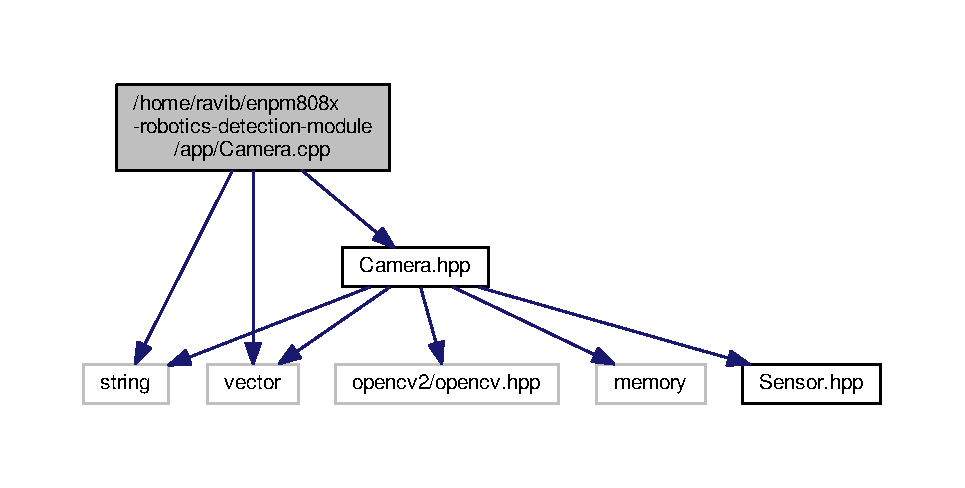
\includegraphics[width=350pt]{_camera_8cpp__incl}
\end{center}
\end{figure}


\subsection{Detailed Description}
\begin{DoxyAuthor}{Author}
Ravi Bhadeshiya 
\end{DoxyAuthor}
\begin{DoxyVersion}{Version}
1.\+0 
\end{DoxyVersion}
\begin{DoxyCopyright}{Copyright}
M\+IT License (c) 2017 Ravi Bhadeshiya 
\end{DoxyCopyright}

\hypertarget{_detection_8cpp}{}\section{/home/ravib/enpm808x-\/robotics-\/detection-\/module/app/\+Detection.cpp File Reference}
\label{_detection_8cpp}\index{/home/ravib/enpm808x-\/robotics-\/detection-\/module/app/\+Detection.\+cpp@{/home/ravib/enpm808x-\/robotics-\/detection-\/module/app/\+Detection.\+cpp}}
{\ttfamily \#include $<$boost/range/irange.\+hpp$>$}\newline
{\ttfamily \#include $<$vector$>$}\newline
{\ttfamily \#include \char`\"{}Detection.\+hpp\char`\"{}}\newline
Include dependency graph for Detection.\+cpp\+:
\nopagebreak
\begin{figure}[H]
\begin{center}
\leavevmode
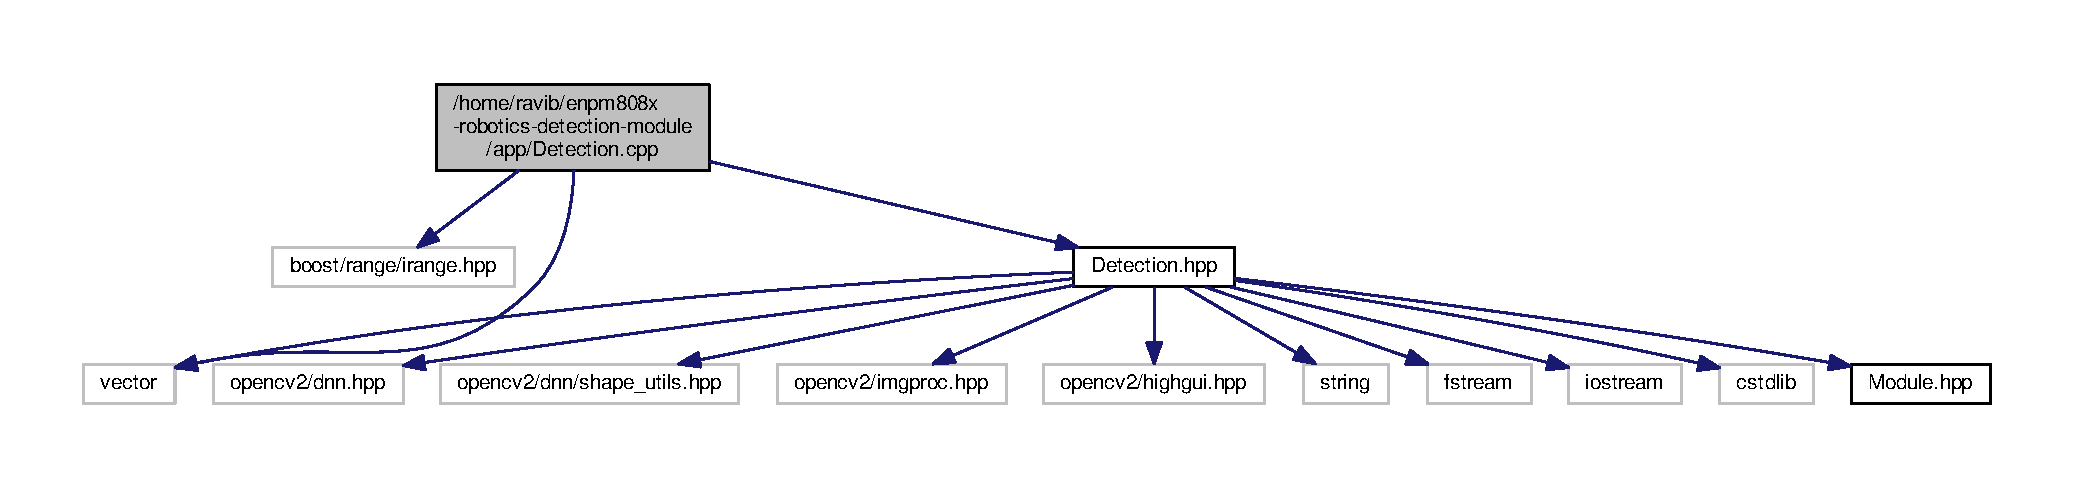
\includegraphics[width=350pt]{_detection_8cpp__incl}
\end{center}
\end{figure}


\subsection{Detailed Description}
\begin{DoxyAuthor}{Author}
Ravi Bhadeshiya 
\end{DoxyAuthor}
\begin{DoxyVersion}{Version}
1.\+0 
\end{DoxyVersion}
\begin{DoxyCopyright}{Copyright}
M\+IT License (c) 2017 Ravi Bhadeshiya 
\end{DoxyCopyright}

\hypertarget{app_2main_8cpp}{}\section{/home/ravib/enpm808x-\/robotics-\/detection-\/module/app/main.cpp File Reference}
\label{app_2main_8cpp}\index{/home/ravib/enpm808x-\/robotics-\/detection-\/module/app/main.\+cpp@{/home/ravib/enpm808x-\/robotics-\/detection-\/module/app/main.\+cpp}}
{\ttfamily \#include $<$iostream$>$}\newline
{\ttfamily \#include $<$memory$>$}\newline
{\ttfamily \#include $<$string$>$}\newline
{\ttfamily \#include \char`\"{}Robot.\+hpp\char`\"{}}\newline
Include dependency graph for main.\+cpp\+:
\nopagebreak
\begin{figure}[H]
\begin{center}
\leavevmode
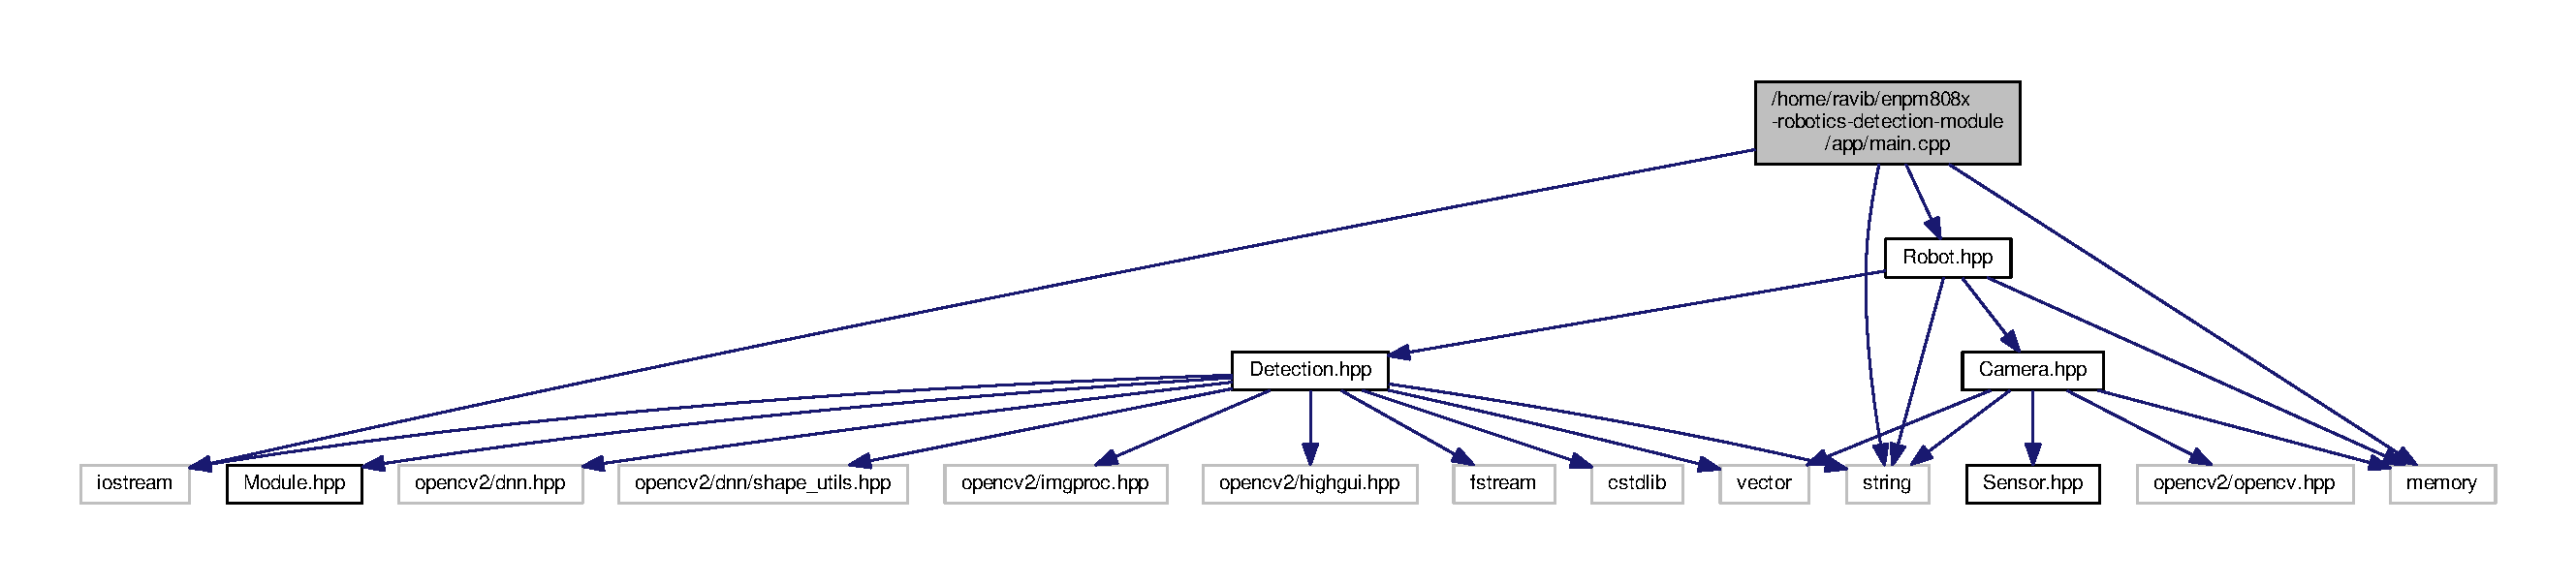
\includegraphics[width=350pt]{app_2main_8cpp__incl}
\end{center}
\end{figure}
\subsection*{Functions}
\begin{DoxyCompactItemize}
\item 
int \hyperlink{app_2main_8cpp_a0ddf1224851353fc92bfbff6f499fa97}{main} (int argc, char $\ast$argv\mbox{[}$\,$\mbox{]})
\begin{DoxyCompactList}\small\item\em Main function. \end{DoxyCompactList}\end{DoxyCompactItemize}


\subsection{Function Documentation}
\mbox{\Hypertarget{app_2main_8cpp_a0ddf1224851353fc92bfbff6f499fa97}\label{app_2main_8cpp_a0ddf1224851353fc92bfbff6f499fa97}} 
\index{app/main.\+cpp@{app/main.\+cpp}!main@{main}}
\index{main@{main}!app/main.\+cpp@{app/main.\+cpp}}
\subsubsection{\texorpdfstring{main()}{main()}}
{\footnotesize\ttfamily int main (\begin{DoxyParamCaption}\item[{int}]{argc,  }\item[{char $\ast$}]{argv\mbox{[}$\,$\mbox{]} }\end{DoxyParamCaption})}



Main function. 

\begin{DoxyReturn}{Returns}
return zero if run properly 
\end{DoxyReturn}


Definition at line 20 of file main.\+cpp.


\hypertarget{test_2main_8cpp}{}\section{/home/ravib/enpm808x-\/robotics-\/detection-\/module/test/main.cpp File Reference}
\label{test_2main_8cpp}\index{/home/ravib/enpm808x-\/robotics-\/detection-\/module/test/main.\+cpp@{/home/ravib/enpm808x-\/robotics-\/detection-\/module/test/main.\+cpp}}
{\ttfamily \#include $<$gtest/gtest.\+h$>$}\newline
Include dependency graph for main.\+cpp\+:
\nopagebreak
\begin{figure}[H]
\begin{center}
\leavevmode
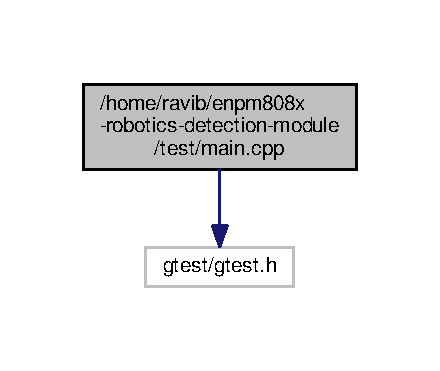
\includegraphics[width=211pt]{test_2main_8cpp__incl}
\end{center}
\end{figure}
\subsection*{Functions}
\begin{DoxyCompactItemize}
\item 
int \hyperlink{test_2main_8cpp_a3c04138a5bfe5d72780bb7e82a18e627}{main} (int argc, char $\ast$$\ast$argv)
\end{DoxyCompactItemize}


\subsection{Function Documentation}
\mbox{\Hypertarget{test_2main_8cpp_a3c04138a5bfe5d72780bb7e82a18e627}\label{test_2main_8cpp_a3c04138a5bfe5d72780bb7e82a18e627}} 
\index{test/main.\+cpp@{test/main.\+cpp}!main@{main}}
\index{main@{main}!test/main.\+cpp@{test/main.\+cpp}}
\subsubsection{\texorpdfstring{main()}{main()}}
{\footnotesize\ttfamily int main (\begin{DoxyParamCaption}\item[{int}]{argc,  }\item[{char $\ast$$\ast$}]{argv }\end{DoxyParamCaption})}



Definition at line 9 of file main.\+cpp.


\hypertarget{_robot_8cpp}{}\section{/home/ravib/enpm808x-\/robotics-\/detection-\/module/app/\+Robot.cpp File Reference}
\label{_robot_8cpp}\index{/home/ravib/enpm808x-\/robotics-\/detection-\/module/app/\+Robot.\+cpp@{/home/ravib/enpm808x-\/robotics-\/detection-\/module/app/\+Robot.\+cpp}}
{\ttfamily \#include $<$memory$>$}\newline
{\ttfamily \#include $<$string$>$}\newline
{\ttfamily \#include \char`\"{}Robot.\+hpp\char`\"{}}\newline
Include dependency graph for Robot.\+cpp\+:
\nopagebreak
\begin{figure}[H]
\begin{center}
\leavevmode
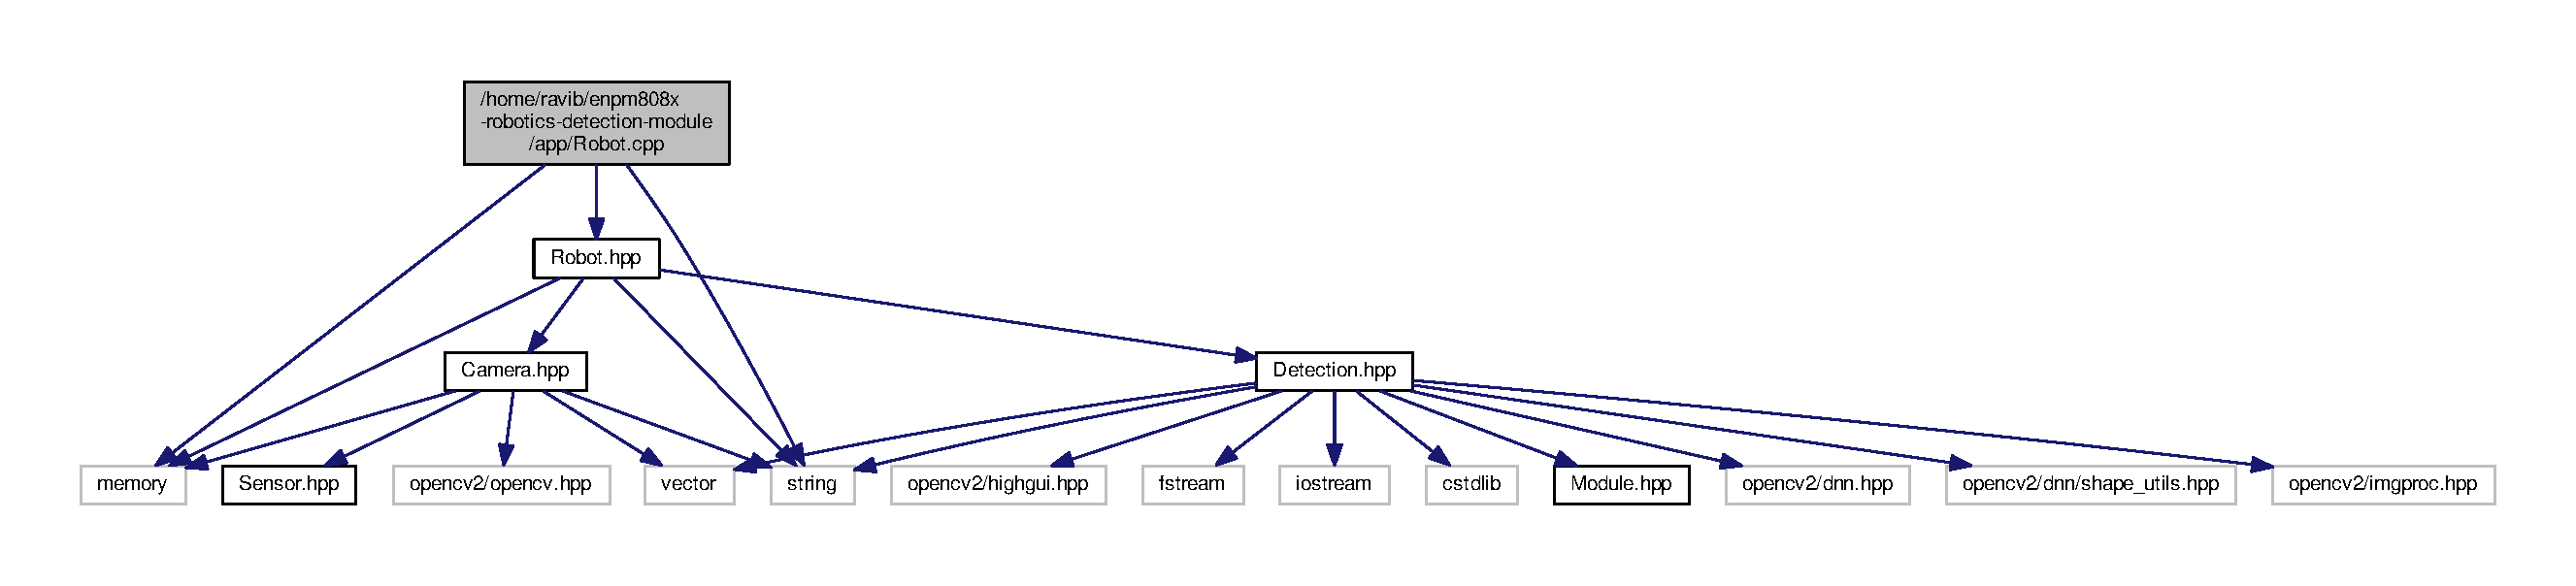
\includegraphics[width=350pt]{_robot_8cpp__incl}
\end{center}
\end{figure}


\subsection{Detailed Description}
\begin{DoxyAuthor}{Author}
Ravi Bhadeshiya 
\end{DoxyAuthor}
\begin{DoxyVersion}{Version}
1.\+0 
\end{DoxyVersion}
\begin{DoxyCopyright}{Copyright}
M\+IT License (c) 2017 Ravi Bhadeshiya 
\end{DoxyCopyright}

\hypertarget{_c_make_c_compiler_id_8c}{}\section{/home/ravib/enpm808x-\/robotics-\/detection-\/module/build/\+C\+Make\+Files/3.5.1/\+Compiler\+Id\+C/\+C\+Make\+C\+Compiler\+Id.c File Reference}
\label{_c_make_c_compiler_id_8c}\index{/home/ravib/enpm808x-\/robotics-\/detection-\/module/build/\+C\+Make\+Files/3.\+5.\+1/\+Compiler\+Id\+C/\+C\+Make\+C\+Compiler\+Id.\+c@{/home/ravib/enpm808x-\/robotics-\/detection-\/module/build/\+C\+Make\+Files/3.\+5.\+1/\+Compiler\+Id\+C/\+C\+Make\+C\+Compiler\+Id.\+c}}
\subsection*{Macros}
\begin{DoxyCompactItemize}
\item 
\#define \hyperlink{_c_make_c_compiler_id_8c_a81dee0709ded976b2e0319239f72d174}{C\+O\+M\+P\+I\+L\+E\+R\+\_\+\+ID}~\char`\"{}\char`\"{}
\item 
\#define \hyperlink{_c_make_c_compiler_id_8c_a2ae9b72bb13abaabfcf2ee0ba7d3fa1d}{S\+T\+R\+I\+N\+G\+I\+F\+Y\+\_\+\+H\+E\+L\+P\+ER}(X)~\#X
\item 
\#define \hyperlink{_c_make_c_compiler_id_8c_a43e1cad902b6477bec893cb6430bd6c8}{S\+T\+R\+I\+N\+G\+I\+FY}(X)~\hyperlink{_c_make_c_x_x_compiler_id_8cpp_a2ae9b72bb13abaabfcf2ee0ba7d3fa1d}{S\+T\+R\+I\+N\+G\+I\+F\+Y\+\_\+\+H\+E\+L\+P\+ER}(X)
\item 
\#define \hyperlink{_c_make_c_compiler_id_8c_adbc5372f40838899018fadbc89bd588b}{P\+L\+A\+T\+F\+O\+R\+M\+\_\+\+ID}~\char`\"{}\char`\"{}
\item 
\#define \hyperlink{_c_make_c_compiler_id_8c_aba35d0d200deaeb06aee95ca297acb28}{A\+R\+C\+H\+I\+T\+E\+C\+T\+U\+R\+E\+\_\+\+ID}~\char`\"{}\char`\"{}
\item 
\#define \hyperlink{_c_make_c_compiler_id_8c_ad1280362da42492bbc11aa78cbf776ad}{D\+EC}(n)
\item 
\#define \hyperlink{_c_make_c_compiler_id_8c_a46d5d95daa1bef867bd0179594310ed5}{H\+EX}(n)
\end{DoxyCompactItemize}
\subsection*{Functions}
\begin{DoxyCompactItemize}
\item 
int \hyperlink{_c_make_c_compiler_id_8c_a0ddf1224851353fc92bfbff6f499fa97}{main} (int argc, char $\ast$argv\mbox{[}$\,$\mbox{]})
\end{DoxyCompactItemize}
\subsection*{Variables}
\begin{DoxyCompactItemize}
\item 
char const  $\ast$ \hyperlink{_c_make_c_compiler_id_8c_a4b0efeb7a5d59313986b3a0390f050f6}{info\+\_\+compiler} = \char`\"{}I\+N\+FO\char`\"{} \char`\"{}\+:\char`\"{} \char`\"{}compiler\mbox{[}\char`\"{} C\+O\+M\+P\+I\+L\+E\+R\+\_\+\+ID \char`\"{}\mbox{]}\char`\"{}
\item 
char const  $\ast$ \hyperlink{_c_make_c_compiler_id_8c_a2321403dee54ee23f0c2fa849c60f7d4}{info\+\_\+platform} = \char`\"{}I\+N\+FO\char`\"{} \char`\"{}\+:\char`\"{} \char`\"{}platform\mbox{[}\char`\"{} P\+L\+A\+T\+F\+O\+R\+M\+\_\+\+ID \char`\"{}\mbox{]}\char`\"{}
\item 
char const  $\ast$ \hyperlink{_c_make_c_compiler_id_8c_a59647e99d304ed33b15cb284c27ed391}{info\+\_\+arch} = \char`\"{}I\+N\+FO\char`\"{} \char`\"{}\+:\char`\"{} \char`\"{}arch\mbox{[}\char`\"{} A\+R\+C\+H\+I\+T\+E\+C\+T\+U\+R\+E\+\_\+\+ID \char`\"{}\mbox{]}\char`\"{}
\item 
const char $\ast$ \hyperlink{_c_make_c_compiler_id_8c_a1ce162bad2fe6966ac8b33cc19e120b8}{info\+\_\+language\+\_\+dialect\+\_\+default}
\end{DoxyCompactItemize}


\subsection{Macro Definition Documentation}
\mbox{\Hypertarget{_c_make_c_compiler_id_8c_aba35d0d200deaeb06aee95ca297acb28}\label{_c_make_c_compiler_id_8c_aba35d0d200deaeb06aee95ca297acb28}} 
\index{C\+Make\+C\+Compiler\+Id.\+c@{C\+Make\+C\+Compiler\+Id.\+c}!A\+R\+C\+H\+I\+T\+E\+C\+T\+U\+R\+E\+\_\+\+ID@{A\+R\+C\+H\+I\+T\+E\+C\+T\+U\+R\+E\+\_\+\+ID}}
\index{A\+R\+C\+H\+I\+T\+E\+C\+T\+U\+R\+E\+\_\+\+ID@{A\+R\+C\+H\+I\+T\+E\+C\+T\+U\+R\+E\+\_\+\+ID}!C\+Make\+C\+Compiler\+Id.\+c@{C\+Make\+C\+Compiler\+Id.\+c}}
\subsubsection{\texorpdfstring{A\+R\+C\+H\+I\+T\+E\+C\+T\+U\+R\+E\+\_\+\+ID}{ARCHITECTURE\_ID}}
{\footnotesize\ttfamily \#define A\+R\+C\+H\+I\+T\+E\+C\+T\+U\+R\+E\+\_\+\+ID~\char`\"{}\char`\"{}}



Definition at line 435 of file C\+Make\+C\+Compiler\+Id.\+c.

\mbox{\Hypertarget{_c_make_c_compiler_id_8c_a81dee0709ded976b2e0319239f72d174}\label{_c_make_c_compiler_id_8c_a81dee0709ded976b2e0319239f72d174}} 
\index{C\+Make\+C\+Compiler\+Id.\+c@{C\+Make\+C\+Compiler\+Id.\+c}!C\+O\+M\+P\+I\+L\+E\+R\+\_\+\+ID@{C\+O\+M\+P\+I\+L\+E\+R\+\_\+\+ID}}
\index{C\+O\+M\+P\+I\+L\+E\+R\+\_\+\+ID@{C\+O\+M\+P\+I\+L\+E\+R\+\_\+\+ID}!C\+Make\+C\+Compiler\+Id.\+c@{C\+Make\+C\+Compiler\+Id.\+c}}
\subsubsection{\texorpdfstring{C\+O\+M\+P\+I\+L\+E\+R\+\_\+\+ID}{COMPILER\_ID}}
{\footnotesize\ttfamily \#define C\+O\+M\+P\+I\+L\+E\+R\+\_\+\+ID~\char`\"{}\char`\"{}}



Definition at line 268 of file C\+Make\+C\+Compiler\+Id.\+c.

\mbox{\Hypertarget{_c_make_c_compiler_id_8c_ad1280362da42492bbc11aa78cbf776ad}\label{_c_make_c_compiler_id_8c_ad1280362da42492bbc11aa78cbf776ad}} 
\index{C\+Make\+C\+Compiler\+Id.\+c@{C\+Make\+C\+Compiler\+Id.\+c}!D\+EC@{D\+EC}}
\index{D\+EC@{D\+EC}!C\+Make\+C\+Compiler\+Id.\+c@{C\+Make\+C\+Compiler\+Id.\+c}}
\subsubsection{\texorpdfstring{D\+EC}{DEC}}
{\footnotesize\ttfamily \#define D\+EC(\begin{DoxyParamCaption}\item[{}]{n }\end{DoxyParamCaption})}

{\bfseries Value\+:}
\begin{DoxyCode}
(\textcolor{charliteral}{'0'} + (((n) / 10000000)%10)), \(\backslash\)
  (\textcolor{charliteral}{'0'} + (((n) / 1000000)%10)),  \(\backslash\)
  (\textcolor{charliteral}{'0'} + (((n) / 100000)%10)),   \(\backslash\)
  (\textcolor{charliteral}{'0'} + (((n) / 10000)%10)),    \(\backslash\)
  (\textcolor{charliteral}{'0'} + (((n) / 1000)%10)),     \(\backslash\)
  (\textcolor{charliteral}{'0'} + (((n) / 100)%10)),      \(\backslash\)
  (\textcolor{charliteral}{'0'} + (((n) / 10)%10)),       \(\backslash\)
  (\textcolor{charliteral}{'0'} +  ((n) % 10))
\end{DoxyCode}


Definition at line 439 of file C\+Make\+C\+Compiler\+Id.\+c.

\mbox{\Hypertarget{_c_make_c_compiler_id_8c_a46d5d95daa1bef867bd0179594310ed5}\label{_c_make_c_compiler_id_8c_a46d5d95daa1bef867bd0179594310ed5}} 
\index{C\+Make\+C\+Compiler\+Id.\+c@{C\+Make\+C\+Compiler\+Id.\+c}!H\+EX@{H\+EX}}
\index{H\+EX@{H\+EX}!C\+Make\+C\+Compiler\+Id.\+c@{C\+Make\+C\+Compiler\+Id.\+c}}
\subsubsection{\texorpdfstring{H\+EX}{HEX}}
{\footnotesize\ttfamily \#define H\+EX(\begin{DoxyParamCaption}\item[{}]{n }\end{DoxyParamCaption})}

{\bfseries Value\+:}
\begin{DoxyCode}
(\textcolor{charliteral}{'0'} + ((n)>>28 & 0xF)), \(\backslash\)
  (\textcolor{charliteral}{'0'} + ((n)>>24 & 0xF)), \(\backslash\)
  (\textcolor{charliteral}{'0'} + ((n)>>20 & 0xF)), \(\backslash\)
  (\textcolor{charliteral}{'0'} + ((n)>>16 & 0xF)), \(\backslash\)
  (\textcolor{charliteral}{'0'} + ((n)>>12 & 0xF)), \(\backslash\)
  (\textcolor{charliteral}{'0'} + ((n)>>8  & 0xF)), \(\backslash\)
  (\textcolor{charliteral}{'0'} + ((n)>>4  & 0xF)), \(\backslash\)
  (\textcolor{charliteral}{'0'} + ((n)     & 0xF))
\end{DoxyCode}


Definition at line 450 of file C\+Make\+C\+Compiler\+Id.\+c.

\mbox{\Hypertarget{_c_make_c_compiler_id_8c_adbc5372f40838899018fadbc89bd588b}\label{_c_make_c_compiler_id_8c_adbc5372f40838899018fadbc89bd588b}} 
\index{C\+Make\+C\+Compiler\+Id.\+c@{C\+Make\+C\+Compiler\+Id.\+c}!P\+L\+A\+T\+F\+O\+R\+M\+\_\+\+ID@{P\+L\+A\+T\+F\+O\+R\+M\+\_\+\+ID}}
\index{P\+L\+A\+T\+F\+O\+R\+M\+\_\+\+ID@{P\+L\+A\+T\+F\+O\+R\+M\+\_\+\+ID}!C\+Make\+C\+Compiler\+Id.\+c@{C\+Make\+C\+Compiler\+Id.\+c}}
\subsubsection{\texorpdfstring{P\+L\+A\+T\+F\+O\+R\+M\+\_\+\+ID}{PLATFORM\_ID}}
{\footnotesize\ttfamily \#define P\+L\+A\+T\+F\+O\+R\+M\+\_\+\+ID~\char`\"{}\char`\"{}}



Definition at line 385 of file C\+Make\+C\+Compiler\+Id.\+c.

\mbox{\Hypertarget{_c_make_c_compiler_id_8c_a43e1cad902b6477bec893cb6430bd6c8}\label{_c_make_c_compiler_id_8c_a43e1cad902b6477bec893cb6430bd6c8}} 
\index{C\+Make\+C\+Compiler\+Id.\+c@{C\+Make\+C\+Compiler\+Id.\+c}!S\+T\+R\+I\+N\+G\+I\+FY@{S\+T\+R\+I\+N\+G\+I\+FY}}
\index{S\+T\+R\+I\+N\+G\+I\+FY@{S\+T\+R\+I\+N\+G\+I\+FY}!C\+Make\+C\+Compiler\+Id.\+c@{C\+Make\+C\+Compiler\+Id.\+c}}
\subsubsection{\texorpdfstring{S\+T\+R\+I\+N\+G\+I\+FY}{STRINGIFY}}
{\footnotesize\ttfamily \#define S\+T\+R\+I\+N\+G\+I\+FY(\begin{DoxyParamCaption}\item[{}]{X }\end{DoxyParamCaption})~\hyperlink{_c_make_c_x_x_compiler_id_8cpp_a2ae9b72bb13abaabfcf2ee0ba7d3fa1d}{S\+T\+R\+I\+N\+G\+I\+F\+Y\+\_\+\+H\+E\+L\+P\+ER}(X)}



Definition at line 289 of file C\+Make\+C\+Compiler\+Id.\+c.

\mbox{\Hypertarget{_c_make_c_compiler_id_8c_a2ae9b72bb13abaabfcf2ee0ba7d3fa1d}\label{_c_make_c_compiler_id_8c_a2ae9b72bb13abaabfcf2ee0ba7d3fa1d}} 
\index{C\+Make\+C\+Compiler\+Id.\+c@{C\+Make\+C\+Compiler\+Id.\+c}!S\+T\+R\+I\+N\+G\+I\+F\+Y\+\_\+\+H\+E\+L\+P\+ER@{S\+T\+R\+I\+N\+G\+I\+F\+Y\+\_\+\+H\+E\+L\+P\+ER}}
\index{S\+T\+R\+I\+N\+G\+I\+F\+Y\+\_\+\+H\+E\+L\+P\+ER@{S\+T\+R\+I\+N\+G\+I\+F\+Y\+\_\+\+H\+E\+L\+P\+ER}!C\+Make\+C\+Compiler\+Id.\+c@{C\+Make\+C\+Compiler\+Id.\+c}}
\subsubsection{\texorpdfstring{S\+T\+R\+I\+N\+G\+I\+F\+Y\+\_\+\+H\+E\+L\+P\+ER}{STRINGIFY\_HELPER}}
{\footnotesize\ttfamily \#define S\+T\+R\+I\+N\+G\+I\+F\+Y\+\_\+\+H\+E\+L\+P\+ER(\begin{DoxyParamCaption}\item[{}]{X }\end{DoxyParamCaption})~\#X}



Definition at line 288 of file C\+Make\+C\+Compiler\+Id.\+c.



\subsection{Function Documentation}
\mbox{\Hypertarget{_c_make_c_compiler_id_8c_a0ddf1224851353fc92bfbff6f499fa97}\label{_c_make_c_compiler_id_8c_a0ddf1224851353fc92bfbff6f499fa97}} 
\index{C\+Make\+C\+Compiler\+Id.\+c@{C\+Make\+C\+Compiler\+Id.\+c}!main@{main}}
\index{main@{main}!C\+Make\+C\+Compiler\+Id.\+c@{C\+Make\+C\+Compiler\+Id.\+c}}
\subsubsection{\texorpdfstring{main()}{main()}}
{\footnotesize\ttfamily int main (\begin{DoxyParamCaption}\item[{int}]{argc,  }\item[{char $\ast$}]{argv\mbox{[}$\,$\mbox{]} }\end{DoxyParamCaption})}



Definition at line 522 of file C\+Make\+C\+Compiler\+Id.\+c.



\subsection{Variable Documentation}
\mbox{\Hypertarget{_c_make_c_compiler_id_8c_a59647e99d304ed33b15cb284c27ed391}\label{_c_make_c_compiler_id_8c_a59647e99d304ed33b15cb284c27ed391}} 
\index{C\+Make\+C\+Compiler\+Id.\+c@{C\+Make\+C\+Compiler\+Id.\+c}!info\+\_\+arch@{info\+\_\+arch}}
\index{info\+\_\+arch@{info\+\_\+arch}!C\+Make\+C\+Compiler\+Id.\+c@{C\+Make\+C\+Compiler\+Id.\+c}}
\subsubsection{\texorpdfstring{info\+\_\+arch}{info\_arch}}
{\footnotesize\ttfamily char const$\ast$ info\+\_\+arch = \char`\"{}I\+N\+FO\char`\"{} \char`\"{}\+:\char`\"{} \char`\"{}arch\mbox{[}\char`\"{} A\+R\+C\+H\+I\+T\+E\+C\+T\+U\+R\+E\+\_\+\+ID \char`\"{}\mbox{]}\char`\"{}}



Definition at line 501 of file C\+Make\+C\+Compiler\+Id.\+c.

\mbox{\Hypertarget{_c_make_c_compiler_id_8c_a4b0efeb7a5d59313986b3a0390f050f6}\label{_c_make_c_compiler_id_8c_a4b0efeb7a5d59313986b3a0390f050f6}} 
\index{C\+Make\+C\+Compiler\+Id.\+c@{C\+Make\+C\+Compiler\+Id.\+c}!info\+\_\+compiler@{info\+\_\+compiler}}
\index{info\+\_\+compiler@{info\+\_\+compiler}!C\+Make\+C\+Compiler\+Id.\+c@{C\+Make\+C\+Compiler\+Id.\+c}}
\subsubsection{\texorpdfstring{info\+\_\+compiler}{info\_compiler}}
{\footnotesize\ttfamily char const$\ast$ info\+\_\+compiler = \char`\"{}I\+N\+FO\char`\"{} \char`\"{}\+:\char`\"{} \char`\"{}compiler\mbox{[}\char`\"{} C\+O\+M\+P\+I\+L\+E\+R\+\_\+\+ID \char`\"{}\mbox{]}\char`\"{}}



Definition at line 275 of file C\+Make\+C\+Compiler\+Id.\+c.

\mbox{\Hypertarget{_c_make_c_compiler_id_8c_a1ce162bad2fe6966ac8b33cc19e120b8}\label{_c_make_c_compiler_id_8c_a1ce162bad2fe6966ac8b33cc19e120b8}} 
\index{C\+Make\+C\+Compiler\+Id.\+c@{C\+Make\+C\+Compiler\+Id.\+c}!info\+\_\+language\+\_\+dialect\+\_\+default@{info\+\_\+language\+\_\+dialect\+\_\+default}}
\index{info\+\_\+language\+\_\+dialect\+\_\+default@{info\+\_\+language\+\_\+dialect\+\_\+default}!C\+Make\+C\+Compiler\+Id.\+c@{C\+Make\+C\+Compiler\+Id.\+c}}
\subsubsection{\texorpdfstring{info\+\_\+language\+\_\+dialect\+\_\+default}{info\_language\_dialect\_default}}
{\footnotesize\ttfamily const char$\ast$ info\+\_\+language\+\_\+dialect\+\_\+default}

{\bfseries Initial value\+:}
\begin{DoxyCode}
= \textcolor{stringliteral}{"INFO"} \textcolor{stringliteral}{":"} \textcolor{stringliteral}{"dialect\_default["}

  \textcolor{stringliteral}{"90"}






\textcolor{stringliteral}{"]"}
\end{DoxyCode}


Definition at line 506 of file C\+Make\+C\+Compiler\+Id.\+c.

\mbox{\Hypertarget{_c_make_c_compiler_id_8c_a2321403dee54ee23f0c2fa849c60f7d4}\label{_c_make_c_compiler_id_8c_a2321403dee54ee23f0c2fa849c60f7d4}} 
\index{C\+Make\+C\+Compiler\+Id.\+c@{C\+Make\+C\+Compiler\+Id.\+c}!info\+\_\+platform@{info\+\_\+platform}}
\index{info\+\_\+platform@{info\+\_\+platform}!C\+Make\+C\+Compiler\+Id.\+c@{C\+Make\+C\+Compiler\+Id.\+c}}
\subsubsection{\texorpdfstring{info\+\_\+platform}{info\_platform}}
{\footnotesize\ttfamily char const$\ast$ info\+\_\+platform = \char`\"{}I\+N\+FO\char`\"{} \char`\"{}\+:\char`\"{} \char`\"{}platform\mbox{[}\char`\"{} P\+L\+A\+T\+F\+O\+R\+M\+\_\+\+ID \char`\"{}\mbox{]}\char`\"{}}



Definition at line 500 of file C\+Make\+C\+Compiler\+Id.\+c.


\hypertarget{_c_make_c_x_x_compiler_id_8cpp}{}\section{/home/ravib/enpm808x-\/robotics-\/detection-\/module/build/\+C\+Make\+Files/3.5.1/\+Compiler\+Id\+C\+X\+X/\+C\+Make\+C\+X\+X\+Compiler\+Id.cpp File Reference}
\label{_c_make_c_x_x_compiler_id_8cpp}\index{/home/ravib/enpm808x-\/robotics-\/detection-\/module/build/\+C\+Make\+Files/3.\+5.\+1/\+Compiler\+Id\+C\+X\+X/\+C\+Make\+C\+X\+X\+Compiler\+Id.\+cpp@{/home/ravib/enpm808x-\/robotics-\/detection-\/module/build/\+C\+Make\+Files/3.\+5.\+1/\+Compiler\+Id\+C\+X\+X/\+C\+Make\+C\+X\+X\+Compiler\+Id.\+cpp}}
\subsection*{Macros}
\begin{DoxyCompactItemize}
\item 
\#define \hyperlink{_c_make_c_x_x_compiler_id_8cpp_a81dee0709ded976b2e0319239f72d174}{C\+O\+M\+P\+I\+L\+E\+R\+\_\+\+ID}~\char`\"{}\char`\"{}
\item 
\#define \hyperlink{_c_make_c_x_x_compiler_id_8cpp_a2ae9b72bb13abaabfcf2ee0ba7d3fa1d}{S\+T\+R\+I\+N\+G\+I\+F\+Y\+\_\+\+H\+E\+L\+P\+ER}(X)~\#X
\item 
\#define \hyperlink{_c_make_c_x_x_compiler_id_8cpp_a43e1cad902b6477bec893cb6430bd6c8}{S\+T\+R\+I\+N\+G\+I\+FY}(X)~\hyperlink{_c_make_c_x_x_compiler_id_8cpp_a2ae9b72bb13abaabfcf2ee0ba7d3fa1d}{S\+T\+R\+I\+N\+G\+I\+F\+Y\+\_\+\+H\+E\+L\+P\+ER}(X)
\item 
\#define \hyperlink{_c_make_c_x_x_compiler_id_8cpp_adbc5372f40838899018fadbc89bd588b}{P\+L\+A\+T\+F\+O\+R\+M\+\_\+\+ID}~\char`\"{}\char`\"{}
\item 
\#define \hyperlink{_c_make_c_x_x_compiler_id_8cpp_aba35d0d200deaeb06aee95ca297acb28}{A\+R\+C\+H\+I\+T\+E\+C\+T\+U\+R\+E\+\_\+\+ID}~\char`\"{}\char`\"{}
\item 
\#define \hyperlink{_c_make_c_x_x_compiler_id_8cpp_ad1280362da42492bbc11aa78cbf776ad}{D\+EC}(n)
\item 
\#define \hyperlink{_c_make_c_x_x_compiler_id_8cpp_a46d5d95daa1bef867bd0179594310ed5}{H\+EX}(n)
\end{DoxyCompactItemize}
\subsection*{Functions}
\begin{DoxyCompactItemize}
\item 
int \hyperlink{_c_make_c_x_x_compiler_id_8cpp_a0ddf1224851353fc92bfbff6f499fa97}{main} (int argc, char $\ast$argv\mbox{[}$\,$\mbox{]})
\end{DoxyCompactItemize}
\subsection*{Variables}
\begin{DoxyCompactItemize}
\item 
char const  $\ast$ \hyperlink{_c_make_c_x_x_compiler_id_8cpp_a4b0efeb7a5d59313986b3a0390f050f6}{info\+\_\+compiler} = \char`\"{}I\+N\+FO\char`\"{} \char`\"{}\+:\char`\"{} \char`\"{}compiler\mbox{[}\char`\"{} C\+O\+M\+P\+I\+L\+E\+R\+\_\+\+ID \char`\"{}\mbox{]}\char`\"{}
\item 
char const  $\ast$ \hyperlink{_c_make_c_x_x_compiler_id_8cpp_a2321403dee54ee23f0c2fa849c60f7d4}{info\+\_\+platform} = \char`\"{}I\+N\+FO\char`\"{} \char`\"{}\+:\char`\"{} \char`\"{}platform\mbox{[}\char`\"{} P\+L\+A\+T\+F\+O\+R\+M\+\_\+\+ID \char`\"{}\mbox{]}\char`\"{}
\item 
char const  $\ast$ \hyperlink{_c_make_c_x_x_compiler_id_8cpp_a59647e99d304ed33b15cb284c27ed391}{info\+\_\+arch} = \char`\"{}I\+N\+FO\char`\"{} \char`\"{}\+:\char`\"{} \char`\"{}arch\mbox{[}\char`\"{} A\+R\+C\+H\+I\+T\+E\+C\+T\+U\+R\+E\+\_\+\+ID \char`\"{}\mbox{]}\char`\"{}
\item 
const char $\ast$ \hyperlink{_c_make_c_x_x_compiler_id_8cpp_a1ce162bad2fe6966ac8b33cc19e120b8}{info\+\_\+language\+\_\+dialect\+\_\+default}
\end{DoxyCompactItemize}


\subsection{Macro Definition Documentation}
\mbox{\Hypertarget{_c_make_c_x_x_compiler_id_8cpp_aba35d0d200deaeb06aee95ca297acb28}\label{_c_make_c_x_x_compiler_id_8cpp_aba35d0d200deaeb06aee95ca297acb28}} 
\index{C\+Make\+C\+X\+X\+Compiler\+Id.\+cpp@{C\+Make\+C\+X\+X\+Compiler\+Id.\+cpp}!A\+R\+C\+H\+I\+T\+E\+C\+T\+U\+R\+E\+\_\+\+ID@{A\+R\+C\+H\+I\+T\+E\+C\+T\+U\+R\+E\+\_\+\+ID}}
\index{A\+R\+C\+H\+I\+T\+E\+C\+T\+U\+R\+E\+\_\+\+ID@{A\+R\+C\+H\+I\+T\+E\+C\+T\+U\+R\+E\+\_\+\+ID}!C\+Make\+C\+X\+X\+Compiler\+Id.\+cpp@{C\+Make\+C\+X\+X\+Compiler\+Id.\+cpp}}
\subsubsection{\texorpdfstring{A\+R\+C\+H\+I\+T\+E\+C\+T\+U\+R\+E\+\_\+\+ID}{ARCHITECTURE\_ID}}
{\footnotesize\ttfamily \#define A\+R\+C\+H\+I\+T\+E\+C\+T\+U\+R\+E\+\_\+\+ID~\char`\"{}\char`\"{}}



Definition at line 430 of file C\+Make\+C\+X\+X\+Compiler\+Id.\+cpp.

\mbox{\Hypertarget{_c_make_c_x_x_compiler_id_8cpp_a81dee0709ded976b2e0319239f72d174}\label{_c_make_c_x_x_compiler_id_8cpp_a81dee0709ded976b2e0319239f72d174}} 
\index{C\+Make\+C\+X\+X\+Compiler\+Id.\+cpp@{C\+Make\+C\+X\+X\+Compiler\+Id.\+cpp}!C\+O\+M\+P\+I\+L\+E\+R\+\_\+\+ID@{C\+O\+M\+P\+I\+L\+E\+R\+\_\+\+ID}}
\index{C\+O\+M\+P\+I\+L\+E\+R\+\_\+\+ID@{C\+O\+M\+P\+I\+L\+E\+R\+\_\+\+ID}!C\+Make\+C\+X\+X\+Compiler\+Id.\+cpp@{C\+Make\+C\+X\+X\+Compiler\+Id.\+cpp}}
\subsubsection{\texorpdfstring{C\+O\+M\+P\+I\+L\+E\+R\+\_\+\+ID}{COMPILER\_ID}}
{\footnotesize\ttfamily \#define C\+O\+M\+P\+I\+L\+E\+R\+\_\+\+ID~\char`\"{}\char`\"{}}



Definition at line 263 of file C\+Make\+C\+X\+X\+Compiler\+Id.\+cpp.

\mbox{\Hypertarget{_c_make_c_x_x_compiler_id_8cpp_ad1280362da42492bbc11aa78cbf776ad}\label{_c_make_c_x_x_compiler_id_8cpp_ad1280362da42492bbc11aa78cbf776ad}} 
\index{C\+Make\+C\+X\+X\+Compiler\+Id.\+cpp@{C\+Make\+C\+X\+X\+Compiler\+Id.\+cpp}!D\+EC@{D\+EC}}
\index{D\+EC@{D\+EC}!C\+Make\+C\+X\+X\+Compiler\+Id.\+cpp@{C\+Make\+C\+X\+X\+Compiler\+Id.\+cpp}}
\subsubsection{\texorpdfstring{D\+EC}{DEC}}
{\footnotesize\ttfamily \#define D\+EC(\begin{DoxyParamCaption}\item[{}]{n }\end{DoxyParamCaption})}

{\bfseries Value\+:}
\begin{DoxyCode}
(\textcolor{charliteral}{'0'} + (((n) / 10000000)%10)), \(\backslash\)
  (\textcolor{charliteral}{'0'} + (((n) / 1000000)%10)),  \(\backslash\)
  (\textcolor{charliteral}{'0'} + (((n) / 100000)%10)),   \(\backslash\)
  (\textcolor{charliteral}{'0'} + (((n) / 10000)%10)),    \(\backslash\)
  (\textcolor{charliteral}{'0'} + (((n) / 1000)%10)),     \(\backslash\)
  (\textcolor{charliteral}{'0'} + (((n) / 100)%10)),      \(\backslash\)
  (\textcolor{charliteral}{'0'} + (((n) / 10)%10)),       \(\backslash\)
  (\textcolor{charliteral}{'0'} +  ((n) % 10))
\end{DoxyCode}


Definition at line 434 of file C\+Make\+C\+X\+X\+Compiler\+Id.\+cpp.

\mbox{\Hypertarget{_c_make_c_x_x_compiler_id_8cpp_a46d5d95daa1bef867bd0179594310ed5}\label{_c_make_c_x_x_compiler_id_8cpp_a46d5d95daa1bef867bd0179594310ed5}} 
\index{C\+Make\+C\+X\+X\+Compiler\+Id.\+cpp@{C\+Make\+C\+X\+X\+Compiler\+Id.\+cpp}!H\+EX@{H\+EX}}
\index{H\+EX@{H\+EX}!C\+Make\+C\+X\+X\+Compiler\+Id.\+cpp@{C\+Make\+C\+X\+X\+Compiler\+Id.\+cpp}}
\subsubsection{\texorpdfstring{H\+EX}{HEX}}
{\footnotesize\ttfamily \#define H\+EX(\begin{DoxyParamCaption}\item[{}]{n }\end{DoxyParamCaption})}

{\bfseries Value\+:}
\begin{DoxyCode}
(\textcolor{charliteral}{'0'} + ((n)>>28 & 0xF)), \(\backslash\)
  (\textcolor{charliteral}{'0'} + ((n)>>24 & 0xF)), \(\backslash\)
  (\textcolor{charliteral}{'0'} + ((n)>>20 & 0xF)), \(\backslash\)
  (\textcolor{charliteral}{'0'} + ((n)>>16 & 0xF)), \(\backslash\)
  (\textcolor{charliteral}{'0'} + ((n)>>12 & 0xF)), \(\backslash\)
  (\textcolor{charliteral}{'0'} + ((n)>>8  & 0xF)), \(\backslash\)
  (\textcolor{charliteral}{'0'} + ((n)>>4  & 0xF)), \(\backslash\)
  (\textcolor{charliteral}{'0'} + ((n)     & 0xF))
\end{DoxyCode}


Definition at line 445 of file C\+Make\+C\+X\+X\+Compiler\+Id.\+cpp.

\mbox{\Hypertarget{_c_make_c_x_x_compiler_id_8cpp_adbc5372f40838899018fadbc89bd588b}\label{_c_make_c_x_x_compiler_id_8cpp_adbc5372f40838899018fadbc89bd588b}} 
\index{C\+Make\+C\+X\+X\+Compiler\+Id.\+cpp@{C\+Make\+C\+X\+X\+Compiler\+Id.\+cpp}!P\+L\+A\+T\+F\+O\+R\+M\+\_\+\+ID@{P\+L\+A\+T\+F\+O\+R\+M\+\_\+\+ID}}
\index{P\+L\+A\+T\+F\+O\+R\+M\+\_\+\+ID@{P\+L\+A\+T\+F\+O\+R\+M\+\_\+\+ID}!C\+Make\+C\+X\+X\+Compiler\+Id.\+cpp@{C\+Make\+C\+X\+X\+Compiler\+Id.\+cpp}}
\subsubsection{\texorpdfstring{P\+L\+A\+T\+F\+O\+R\+M\+\_\+\+ID}{PLATFORM\_ID}}
{\footnotesize\ttfamily \#define P\+L\+A\+T\+F\+O\+R\+M\+\_\+\+ID~\char`\"{}\char`\"{}}



Definition at line 380 of file C\+Make\+C\+X\+X\+Compiler\+Id.\+cpp.

\mbox{\Hypertarget{_c_make_c_x_x_compiler_id_8cpp_a43e1cad902b6477bec893cb6430bd6c8}\label{_c_make_c_x_x_compiler_id_8cpp_a43e1cad902b6477bec893cb6430bd6c8}} 
\index{C\+Make\+C\+X\+X\+Compiler\+Id.\+cpp@{C\+Make\+C\+X\+X\+Compiler\+Id.\+cpp}!S\+T\+R\+I\+N\+G\+I\+FY@{S\+T\+R\+I\+N\+G\+I\+FY}}
\index{S\+T\+R\+I\+N\+G\+I\+FY@{S\+T\+R\+I\+N\+G\+I\+FY}!C\+Make\+C\+X\+X\+Compiler\+Id.\+cpp@{C\+Make\+C\+X\+X\+Compiler\+Id.\+cpp}}
\subsubsection{\texorpdfstring{S\+T\+R\+I\+N\+G\+I\+FY}{STRINGIFY}}
{\footnotesize\ttfamily \#define S\+T\+R\+I\+N\+G\+I\+FY(\begin{DoxyParamCaption}\item[{}]{X }\end{DoxyParamCaption})~\hyperlink{_c_make_c_x_x_compiler_id_8cpp_a2ae9b72bb13abaabfcf2ee0ba7d3fa1d}{S\+T\+R\+I\+N\+G\+I\+F\+Y\+\_\+\+H\+E\+L\+P\+ER}(X)}



Definition at line 284 of file C\+Make\+C\+X\+X\+Compiler\+Id.\+cpp.

\mbox{\Hypertarget{_c_make_c_x_x_compiler_id_8cpp_a2ae9b72bb13abaabfcf2ee0ba7d3fa1d}\label{_c_make_c_x_x_compiler_id_8cpp_a2ae9b72bb13abaabfcf2ee0ba7d3fa1d}} 
\index{C\+Make\+C\+X\+X\+Compiler\+Id.\+cpp@{C\+Make\+C\+X\+X\+Compiler\+Id.\+cpp}!S\+T\+R\+I\+N\+G\+I\+F\+Y\+\_\+\+H\+E\+L\+P\+ER@{S\+T\+R\+I\+N\+G\+I\+F\+Y\+\_\+\+H\+E\+L\+P\+ER}}
\index{S\+T\+R\+I\+N\+G\+I\+F\+Y\+\_\+\+H\+E\+L\+P\+ER@{S\+T\+R\+I\+N\+G\+I\+F\+Y\+\_\+\+H\+E\+L\+P\+ER}!C\+Make\+C\+X\+X\+Compiler\+Id.\+cpp@{C\+Make\+C\+X\+X\+Compiler\+Id.\+cpp}}
\subsubsection{\texorpdfstring{S\+T\+R\+I\+N\+G\+I\+F\+Y\+\_\+\+H\+E\+L\+P\+ER}{STRINGIFY\_HELPER}}
{\footnotesize\ttfamily \#define S\+T\+R\+I\+N\+G\+I\+F\+Y\+\_\+\+H\+E\+L\+P\+ER(\begin{DoxyParamCaption}\item[{}]{X }\end{DoxyParamCaption})~\#X}



Definition at line 283 of file C\+Make\+C\+X\+X\+Compiler\+Id.\+cpp.



\subsection{Function Documentation}
\mbox{\Hypertarget{_c_make_c_x_x_compiler_id_8cpp_a0ddf1224851353fc92bfbff6f499fa97}\label{_c_make_c_x_x_compiler_id_8cpp_a0ddf1224851353fc92bfbff6f499fa97}} 
\index{C\+Make\+C\+X\+X\+Compiler\+Id.\+cpp@{C\+Make\+C\+X\+X\+Compiler\+Id.\+cpp}!main@{main}}
\index{main@{main}!C\+Make\+C\+X\+X\+Compiler\+Id.\+cpp@{C\+Make\+C\+X\+X\+Compiler\+Id.\+cpp}}
\subsubsection{\texorpdfstring{main()}{main()}}
{\footnotesize\ttfamily int main (\begin{DoxyParamCaption}\item[{int}]{argc,  }\item[{char $\ast$}]{argv\mbox{[}$\,$\mbox{]} }\end{DoxyParamCaption})}



Definition at line 513 of file C\+Make\+C\+X\+X\+Compiler\+Id.\+cpp.



\subsection{Variable Documentation}
\mbox{\Hypertarget{_c_make_c_x_x_compiler_id_8cpp_a59647e99d304ed33b15cb284c27ed391}\label{_c_make_c_x_x_compiler_id_8cpp_a59647e99d304ed33b15cb284c27ed391}} 
\index{C\+Make\+C\+X\+X\+Compiler\+Id.\+cpp@{C\+Make\+C\+X\+X\+Compiler\+Id.\+cpp}!info\+\_\+arch@{info\+\_\+arch}}
\index{info\+\_\+arch@{info\+\_\+arch}!C\+Make\+C\+X\+X\+Compiler\+Id.\+cpp@{C\+Make\+C\+X\+X\+Compiler\+Id.\+cpp}}
\subsubsection{\texorpdfstring{info\+\_\+arch}{info\_arch}}
{\footnotesize\ttfamily char const$\ast$ info\+\_\+arch = \char`\"{}I\+N\+FO\char`\"{} \char`\"{}\+:\char`\"{} \char`\"{}arch\mbox{[}\char`\"{} A\+R\+C\+H\+I\+T\+E\+C\+T\+U\+R\+E\+\_\+\+ID \char`\"{}\mbox{]}\char`\"{}}



Definition at line 496 of file C\+Make\+C\+X\+X\+Compiler\+Id.\+cpp.

\mbox{\Hypertarget{_c_make_c_x_x_compiler_id_8cpp_a4b0efeb7a5d59313986b3a0390f050f6}\label{_c_make_c_x_x_compiler_id_8cpp_a4b0efeb7a5d59313986b3a0390f050f6}} 
\index{C\+Make\+C\+X\+X\+Compiler\+Id.\+cpp@{C\+Make\+C\+X\+X\+Compiler\+Id.\+cpp}!info\+\_\+compiler@{info\+\_\+compiler}}
\index{info\+\_\+compiler@{info\+\_\+compiler}!C\+Make\+C\+X\+X\+Compiler\+Id.\+cpp@{C\+Make\+C\+X\+X\+Compiler\+Id.\+cpp}}
\subsubsection{\texorpdfstring{info\+\_\+compiler}{info\_compiler}}
{\footnotesize\ttfamily char const$\ast$ info\+\_\+compiler = \char`\"{}I\+N\+FO\char`\"{} \char`\"{}\+:\char`\"{} \char`\"{}compiler\mbox{[}\char`\"{} C\+O\+M\+P\+I\+L\+E\+R\+\_\+\+ID \char`\"{}\mbox{]}\char`\"{}}



Definition at line 270 of file C\+Make\+C\+X\+X\+Compiler\+Id.\+cpp.

\mbox{\Hypertarget{_c_make_c_x_x_compiler_id_8cpp_a1ce162bad2fe6966ac8b33cc19e120b8}\label{_c_make_c_x_x_compiler_id_8cpp_a1ce162bad2fe6966ac8b33cc19e120b8}} 
\index{C\+Make\+C\+X\+X\+Compiler\+Id.\+cpp@{C\+Make\+C\+X\+X\+Compiler\+Id.\+cpp}!info\+\_\+language\+\_\+dialect\+\_\+default@{info\+\_\+language\+\_\+dialect\+\_\+default}}
\index{info\+\_\+language\+\_\+dialect\+\_\+default@{info\+\_\+language\+\_\+dialect\+\_\+default}!C\+Make\+C\+X\+X\+Compiler\+Id.\+cpp@{C\+Make\+C\+X\+X\+Compiler\+Id.\+cpp}}
\subsubsection{\texorpdfstring{info\+\_\+language\+\_\+dialect\+\_\+default}{info\_language\_dialect\_default}}
{\footnotesize\ttfamily const char$\ast$ info\+\_\+language\+\_\+dialect\+\_\+default}

{\bfseries Initial value\+:}
\begin{DoxyCode}
= \textcolor{stringliteral}{"INFO"} \textcolor{stringliteral}{":"} \textcolor{stringliteral}{"dialect\_default["}





  \textcolor{stringliteral}{"98"}

\textcolor{stringliteral}{"]"}
\end{DoxyCode}


Definition at line 501 of file C\+Make\+C\+X\+X\+Compiler\+Id.\+cpp.

\mbox{\Hypertarget{_c_make_c_x_x_compiler_id_8cpp_a2321403dee54ee23f0c2fa849c60f7d4}\label{_c_make_c_x_x_compiler_id_8cpp_a2321403dee54ee23f0c2fa849c60f7d4}} 
\index{C\+Make\+C\+X\+X\+Compiler\+Id.\+cpp@{C\+Make\+C\+X\+X\+Compiler\+Id.\+cpp}!info\+\_\+platform@{info\+\_\+platform}}
\index{info\+\_\+platform@{info\+\_\+platform}!C\+Make\+C\+X\+X\+Compiler\+Id.\+cpp@{C\+Make\+C\+X\+X\+Compiler\+Id.\+cpp}}
\subsubsection{\texorpdfstring{info\+\_\+platform}{info\_platform}}
{\footnotesize\ttfamily char const$\ast$ info\+\_\+platform = \char`\"{}I\+N\+FO\char`\"{} \char`\"{}\+:\char`\"{} \char`\"{}platform\mbox{[}\char`\"{} P\+L\+A\+T\+F\+O\+R\+M\+\_\+\+ID \char`\"{}\mbox{]}\char`\"{}}



Definition at line 495 of file C\+Make\+C\+X\+X\+Compiler\+Id.\+cpp.


\hypertarget{feature__tests_8c}{}\section{/home/ravib/enpm808x-\/robotics-\/detection-\/module/build/\+C\+Make\+Files/feature\+\_\+tests.c File Reference}
\label{feature__tests_8c}\index{/home/ravib/enpm808x-\/robotics-\/detection-\/module/build/\+C\+Make\+Files/feature\+\_\+tests.\+c@{/home/ravib/enpm808x-\/robotics-\/detection-\/module/build/\+C\+Make\+Files/feature\+\_\+tests.\+c}}
\subsection*{Functions}
\begin{DoxyCompactItemize}
\item 
int \hyperlink{feature__tests_8c_a3c04138a5bfe5d72780bb7e82a18e627}{main} (int argc, char $\ast$$\ast$argv)
\end{DoxyCompactItemize}
\subsection*{Variables}
\begin{DoxyCompactItemize}
\item 
const char \hyperlink{feature__tests_8c_a1582568e32f689337602a16bf8a5bff0}{features} \mbox{[}$\,$\mbox{]}
\end{DoxyCompactItemize}


\subsection{Function Documentation}
\mbox{\Hypertarget{feature__tests_8c_a3c04138a5bfe5d72780bb7e82a18e627}\label{feature__tests_8c_a3c04138a5bfe5d72780bb7e82a18e627}} 
\index{feature\+\_\+tests.\+c@{feature\+\_\+tests.\+c}!main@{main}}
\index{main@{main}!feature\+\_\+tests.\+c@{feature\+\_\+tests.\+c}}
\subsubsection{\texorpdfstring{main()}{main()}}
{\footnotesize\ttfamily int main (\begin{DoxyParamCaption}\item[{int}]{argc,  }\item[{char $\ast$$\ast$}]{argv }\end{DoxyParamCaption})}



Definition at line 34 of file feature\+\_\+tests.\+c.



\subsection{Variable Documentation}
\mbox{\Hypertarget{feature__tests_8c_a1582568e32f689337602a16bf8a5bff0}\label{feature__tests_8c_a1582568e32f689337602a16bf8a5bff0}} 
\index{feature\+\_\+tests.\+c@{feature\+\_\+tests.\+c}!features@{features}}
\index{features@{features}!feature\+\_\+tests.\+c@{feature\+\_\+tests.\+c}}
\subsubsection{\texorpdfstring{features}{features}}
{\footnotesize\ttfamily const char features\mbox{[}$\,$\mbox{]}}



Definition at line 2 of file feature\+\_\+tests.\+c.


\hypertarget{feature__tests_8cxx}{}\section{/home/ravib/enpm808x-\/robotics-\/detection-\/module/build/\+C\+Make\+Files/feature\+\_\+tests.cxx File Reference}
\label{feature__tests_8cxx}\index{/home/ravib/enpm808x-\/robotics-\/detection-\/module/build/\+C\+Make\+Files/feature\+\_\+tests.\+cxx@{/home/ravib/enpm808x-\/robotics-\/detection-\/module/build/\+C\+Make\+Files/feature\+\_\+tests.\+cxx}}
\subsection*{Functions}
\begin{DoxyCompactItemize}
\item 
int \hyperlink{feature__tests_8cxx_a3c04138a5bfe5d72780bb7e82a18e627}{main} (int argc, char $\ast$$\ast$argv)
\end{DoxyCompactItemize}
\subsection*{Variables}
\begin{DoxyCompactItemize}
\item 
const char \hyperlink{feature__tests_8cxx_a1582568e32f689337602a16bf8a5bff0}{features} \mbox{[}$\,$\mbox{]}
\end{DoxyCompactItemize}


\subsection{Function Documentation}
\mbox{\Hypertarget{feature__tests_8cxx_a3c04138a5bfe5d72780bb7e82a18e627}\label{feature__tests_8cxx_a3c04138a5bfe5d72780bb7e82a18e627}} 
\index{feature\+\_\+tests.\+cxx@{feature\+\_\+tests.\+cxx}!main@{main}}
\index{main@{main}!feature\+\_\+tests.\+cxx@{feature\+\_\+tests.\+cxx}}
\subsubsection{\texorpdfstring{main()}{main()}}
{\footnotesize\ttfamily int main (\begin{DoxyParamCaption}\item[{int}]{argc,  }\item[{char $\ast$$\ast$}]{argv }\end{DoxyParamCaption})}



Definition at line 405 of file feature\+\_\+tests.\+cxx.



\subsection{Variable Documentation}
\mbox{\Hypertarget{feature__tests_8cxx_a1582568e32f689337602a16bf8a5bff0}\label{feature__tests_8cxx_a1582568e32f689337602a16bf8a5bff0}} 
\index{feature\+\_\+tests.\+cxx@{feature\+\_\+tests.\+cxx}!features@{features}}
\index{features@{features}!feature\+\_\+tests.\+cxx@{feature\+\_\+tests.\+cxx}}
\subsubsection{\texorpdfstring{features}{features}}
{\footnotesize\ttfamily const char features\mbox{[}$\,$\mbox{]}}



Definition at line 2 of file feature\+\_\+tests.\+cxx.


\hypertarget{_camera_8hpp}{}\section{/home/ravib/enpm808x-\/robotics-\/detection-\/module/include/\+Camera.hpp File Reference}
\label{_camera_8hpp}\index{/home/ravib/enpm808x-\/robotics-\/detection-\/module/include/\+Camera.\+hpp@{/home/ravib/enpm808x-\/robotics-\/detection-\/module/include/\+Camera.\+hpp}}


robotics\+\_\+detection\+\_\+module  


{\ttfamily \#include $<$opencv2/opencv.\+hpp$>$}\newline
{\ttfamily \#include $<$memory$>$}\newline
{\ttfamily \#include $<$string$>$}\newline
{\ttfamily \#include $<$vector$>$}\newline
{\ttfamily \#include \char`\"{}Sensor.\+hpp\char`\"{}}\newline
Include dependency graph for Camera.\+hpp\+:
\nopagebreak
\begin{figure}[H]
\begin{center}
\leavevmode
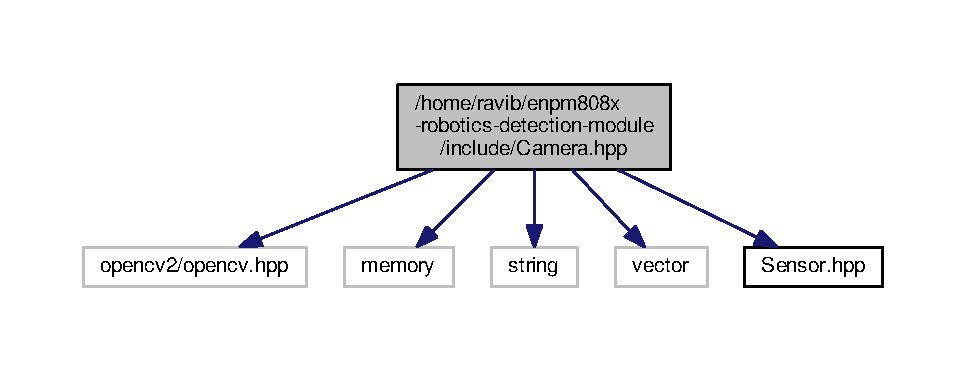
\includegraphics[width=350pt]{_camera_8hpp__incl}
\end{center}
\end{figure}
This graph shows which files directly or indirectly include this file\+:
\nopagebreak
\begin{figure}[H]
\begin{center}
\leavevmode
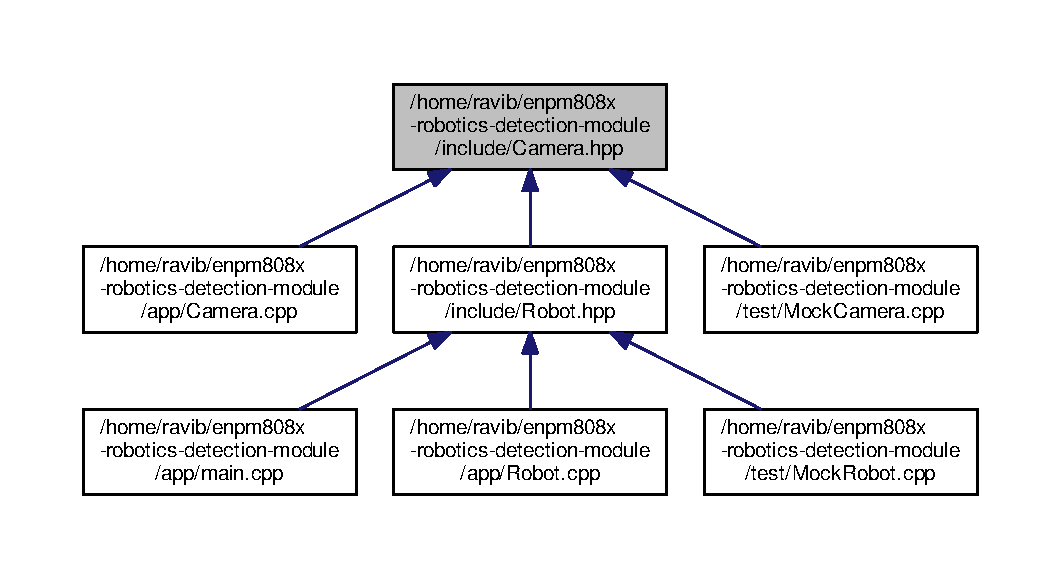
\includegraphics[width=350pt]{_camera_8hpp__dep__incl}
\end{center}
\end{figure}
\subsection*{Classes}
\begin{DoxyCompactItemize}
\item 
class \hyperlink{class_camera}{Camera}
\begin{DoxyCompactList}\small\item\em Class for camera inherited from sensor. \end{DoxyCompactList}\end{DoxyCompactItemize}


\subsection{Detailed Description}
robotics\+\_\+detection\+\_\+module 

\hyperlink{class_camera}{Camera} \hyperlink{class_module}{Module}.

\begin{DoxyAuthor}{Author}
Ravi Bhadeshiya 
\end{DoxyAuthor}
\begin{DoxyVersion}{Version}
1.\+0 
\end{DoxyVersion}
\begin{DoxyCopyright}{Copyright}
M\+IT License (c) 2017 Ravi Bhadeshiya
\end{DoxyCopyright}
\hypertarget{_robot_8hpp_DESCRIPTION}{}\subsection{D\+E\+S\+C\+R\+I\+P\+T\+I\+ON}\label{_robot_8hpp_DESCRIPTION}
This is a little program will run the detection module.

\begin{DoxyAuthor}{Author}
Ravi Bhadeshiya 
\end{DoxyAuthor}
\begin{DoxyVersion}{Version}
1.\+0 
\end{DoxyVersion}
\begin{DoxyCopyright}{Copyright}
M\+IT License (c) 2017 Ravi Bhadeshiya
\end{DoxyCopyright}
\hypertarget{_robot_8hpp_DESCRIPTION}{}\subsection{D\+E\+S\+C\+R\+I\+P\+T\+I\+ON}\label{_robot_8hpp_DESCRIPTION}
This camera module will provide the images for detection by reading jpg/png images or reading a video files.

\begin{DoxyAuthor}{Author}
Ravi Bhadeshiya 
\end{DoxyAuthor}
\begin{DoxyVersion}{Version}
1.\+0 
\end{DoxyVersion}
\begin{DoxyCopyright}{Copyright}
M\+IT License (c) 2017 Ravi Bhadeshiya 
\end{DoxyCopyright}

\hypertarget{_detection_8hpp}{}\section{/home/ravib/enpm808x-\/robotics-\/detection-\/module/include/\+Detection.hpp File Reference}
\label{_detection_8hpp}\index{/home/ravib/enpm808x-\/robotics-\/detection-\/module/include/\+Detection.\+hpp@{/home/ravib/enpm808x-\/robotics-\/detection-\/module/include/\+Detection.\+hpp}}


Deep Nerual Net based \hyperlink{class_detection}{Detection} \hyperlink{class_module}{Module}.  


{\ttfamily \#include $<$opencv2/dnn.\+hpp$>$}\newline
{\ttfamily \#include $<$opencv2/dnn/shape\+\_\+utils.\+hpp$>$}\newline
{\ttfamily \#include $<$opencv2/imgproc.\+hpp$>$}\newline
{\ttfamily \#include $<$opencv2/highgui.\+hpp$>$}\newline
{\ttfamily \#include $<$vector$>$}\newline
{\ttfamily \#include $<$string$>$}\newline
{\ttfamily \#include $<$fstream$>$}\newline
{\ttfamily \#include $<$iostream$>$}\newline
{\ttfamily \#include $<$cstdlib$>$}\newline
{\ttfamily \#include \char`\"{}Module.\+hpp\char`\"{}}\newline
Include dependency graph for Detection.\+hpp\+:
\nopagebreak
\begin{figure}[H]
\begin{center}
\leavevmode
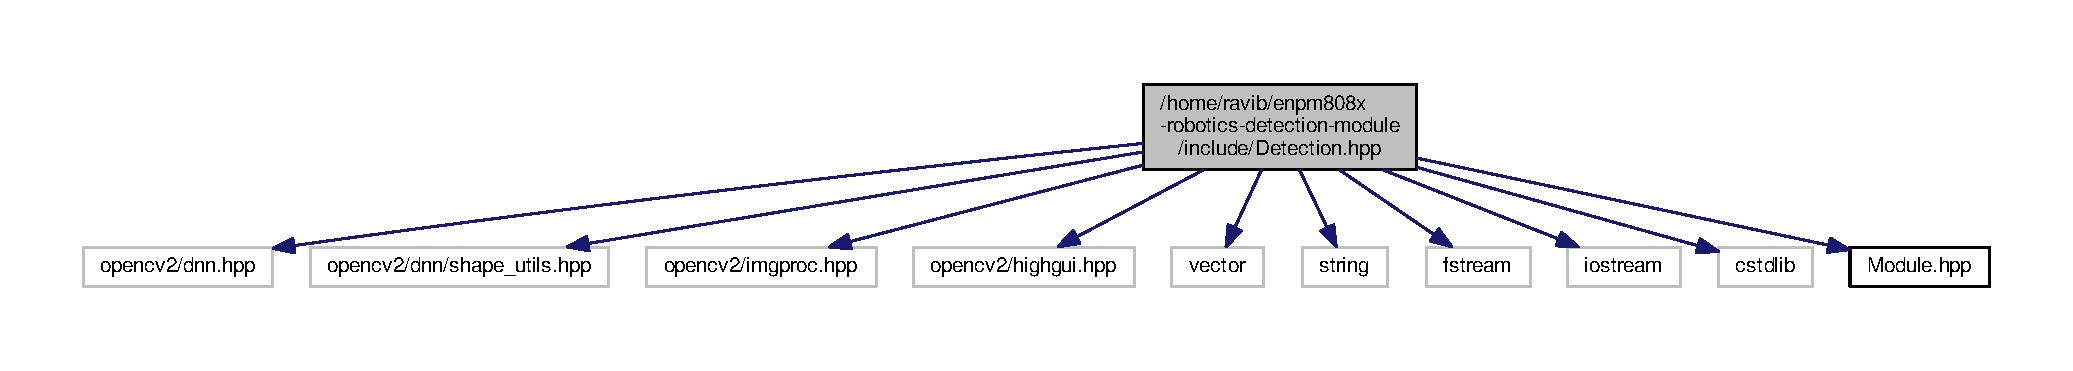
\includegraphics[width=350pt]{_detection_8hpp__incl}
\end{center}
\end{figure}
This graph shows which files directly or indirectly include this file\+:
\nopagebreak
\begin{figure}[H]
\begin{center}
\leavevmode
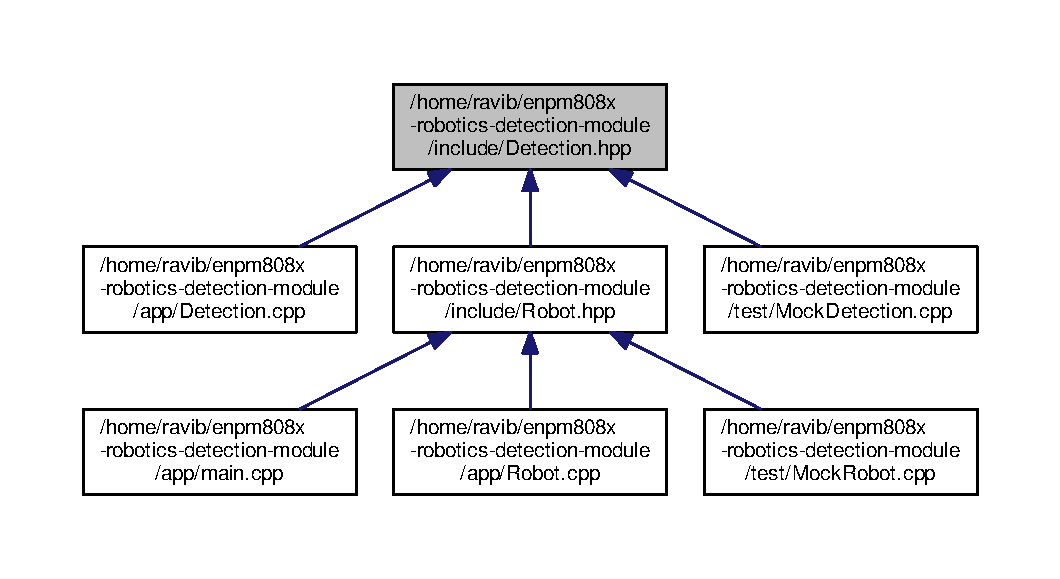
\includegraphics[width=350pt]{_detection_8hpp__dep__incl}
\end{center}
\end{figure}
\subsection*{Classes}
\begin{DoxyCompactItemize}
\item 
class \hyperlink{class_detection}{Detection}
\begin{DoxyCompactList}\small\item\em Class for object detection. \end{DoxyCompactList}\end{DoxyCompactItemize}
\subsection*{Macros}
\begin{DoxyCompactItemize}
\item 
\#define \hyperlink{_detection_8hpp_a9a40981ab5d3bb4701c89a78905e86f8}{D\+E\+B\+U\+G\+\_\+\+D\+E\+T\+C\+T\+I\+ON}
\end{DoxyCompactItemize}


\subsection{Detailed Description}
Deep Nerual Net based \hyperlink{class_detection}{Detection} \hyperlink{class_module}{Module}. 

\begin{DoxyAuthor}{Author}
Ravi Bhadeshiya 
\end{DoxyAuthor}
\begin{DoxyVersion}{Version}
1.\+0 
\end{DoxyVersion}
\begin{DoxyCopyright}{Copyright}
M\+IT License (c) 2017 Ravi Bhadeshiya
\end{DoxyCopyright}
\hypertarget{_robot_8hpp_DESCRIPTION}{}\subsection{D\+E\+S\+C\+R\+I\+P\+T\+I\+ON}\label{_robot_8hpp_DESCRIPTION}
This detection module first preprocess input image and detect multiple object with help of pre-\/trained deep nerual net. The nerual net can be trained for customized image. The deep learning-\/based object detector can process approximately 10-\/15 F\+PS (depending on the speed of your system)

{\bfseries [This]} module uses \href{https://arxiv.org/abs/1512.02325}{\tt Single-\/\+Shot Detector} to detect objects on image. For more info\+: \href{https://github.com/weiliu89/caffe/tree/ssd#models}{\tt Click Here} 

\subsection{Macro Definition Documentation}
\mbox{\Hypertarget{_detection_8hpp_a9a40981ab5d3bb4701c89a78905e86f8}\label{_detection_8hpp_a9a40981ab5d3bb4701c89a78905e86f8}} 
\index{Detection.\+hpp@{Detection.\+hpp}!D\+E\+B\+U\+G\+\_\+\+D\+E\+T\+C\+T\+I\+ON@{D\+E\+B\+U\+G\+\_\+\+D\+E\+T\+C\+T\+I\+ON}}
\index{D\+E\+B\+U\+G\+\_\+\+D\+E\+T\+C\+T\+I\+ON@{D\+E\+B\+U\+G\+\_\+\+D\+E\+T\+C\+T\+I\+ON}!Detection.\+hpp@{Detection.\+hpp}}
\subsubsection{\texorpdfstring{D\+E\+B\+U\+G\+\_\+\+D\+E\+T\+C\+T\+I\+ON}{DEBUG\_DETCTION}}
{\footnotesize\ttfamily \#define D\+E\+B\+U\+G\+\_\+\+D\+E\+T\+C\+T\+I\+ON}



Definition at line 33 of file Detection.\+hpp.


\hypertarget{_module_8hpp}{}\section{/home/ravib/enpm808x-\/robotics-\/detection-\/module/include/\+Module.hpp File Reference}
\label{_module_8hpp}\index{/home/ravib/enpm808x-\/robotics-\/detection-\/module/include/\+Module.\+hpp@{/home/ravib/enpm808x-\/robotics-\/detection-\/module/include/\+Module.\+hpp}}
This graph shows which files directly or indirectly include this file\+:
\nopagebreak
\begin{figure}[H]
\begin{center}
\leavevmode
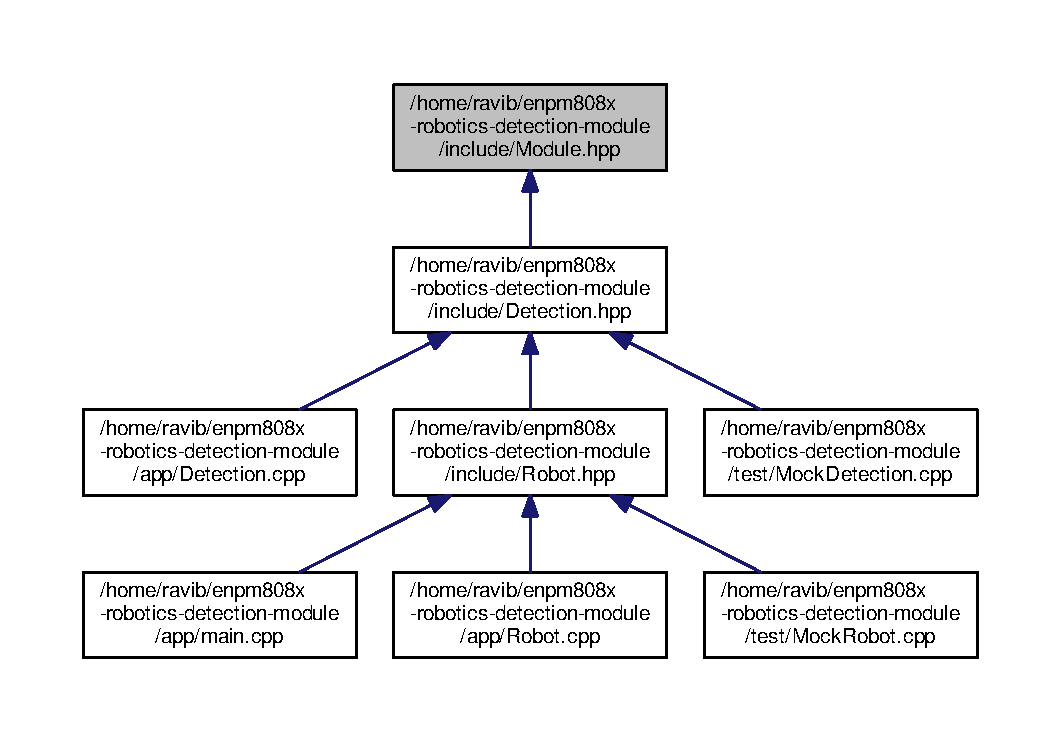
\includegraphics[width=350pt]{_module_8hpp__dep__incl}
\end{center}
\end{figure}
\subsection*{Classes}
\begin{DoxyCompactItemize}
\item 
class \hyperlink{class_module}{Module}
\begin{DoxyCompactList}\small\item\em Virtual Class for detection module. \end{DoxyCompactList}\end{DoxyCompactItemize}


\subsection{Detailed Description}
\begin{DoxyAuthor}{Author}
Ravi Bhadeshiya 
\end{DoxyAuthor}
\begin{DoxyVersion}{Version}
1.\+0 
\end{DoxyVersion}
\begin{DoxyCopyright}{Copyright}
M\+IT License (c) 2017 Ravi Bhadeshiya 
\end{DoxyCopyright}

\hypertarget{_robot_8hpp}{}\section{/home/ravib/enpm808x-\/robotics-\/detection-\/module/include/\+Robot.hpp File Reference}
\label{_robot_8hpp}\index{/home/ravib/enpm808x-\/robotics-\/detection-\/module/include/\+Robot.\+hpp@{/home/ravib/enpm808x-\/robotics-\/detection-\/module/include/\+Robot.\+hpp}}


\hyperlink{class_robot}{Robot} module for handling everthing.  


{\ttfamily \#include $<$memory$>$}\newline
{\ttfamily \#include $<$string$>$}\newline
{\ttfamily \#include \char`\"{}Detection.\+hpp\char`\"{}}\newline
{\ttfamily \#include \char`\"{}Camera.\+hpp\char`\"{}}\newline
Include dependency graph for Robot.\+hpp\+:
\nopagebreak
\begin{figure}[H]
\begin{center}
\leavevmode
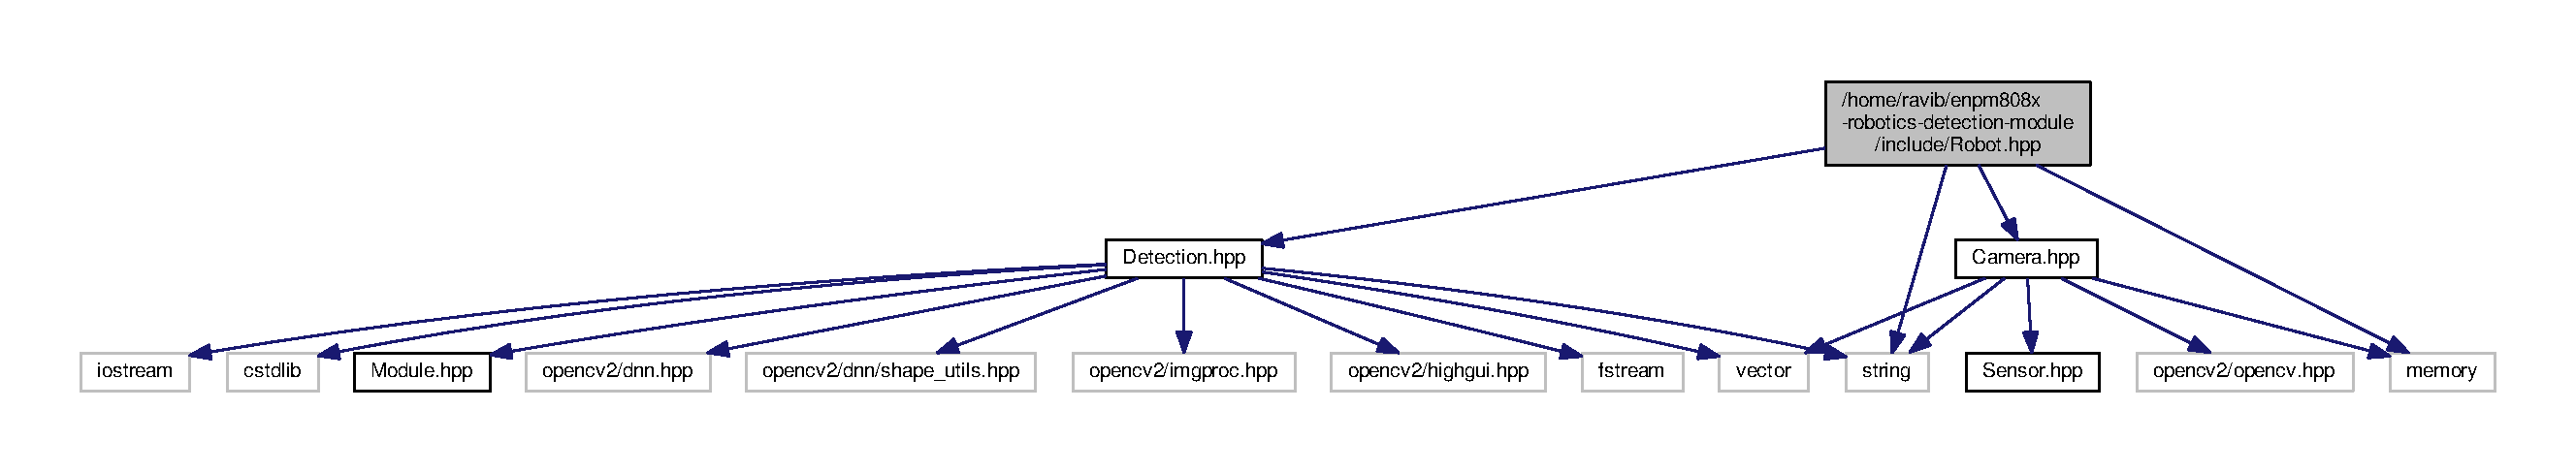
\includegraphics[width=350pt]{_robot_8hpp__incl}
\end{center}
\end{figure}
This graph shows which files directly or indirectly include this file\+:
\nopagebreak
\begin{figure}[H]
\begin{center}
\leavevmode
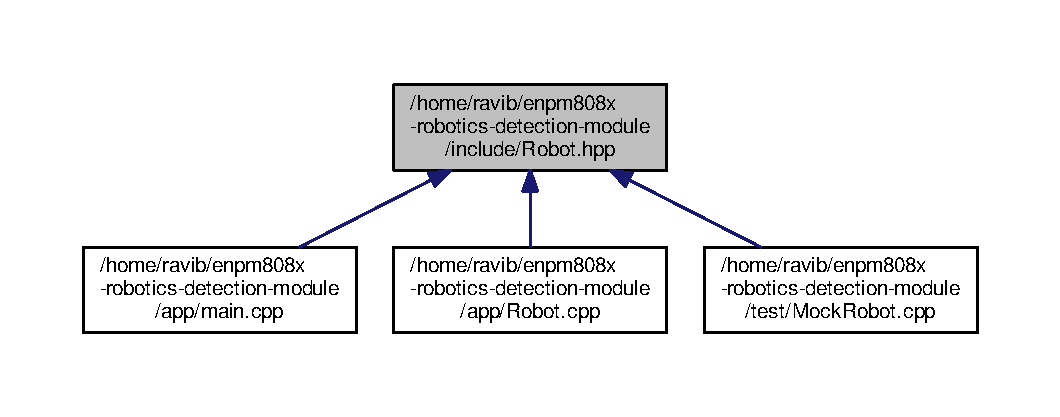
\includegraphics[width=350pt]{_robot_8hpp__dep__incl}
\end{center}
\end{figure}
\subsection*{Classes}
\begin{DoxyCompactItemize}
\item 
class \hyperlink{class_robot}{Robot}
\begin{DoxyCompactList}\small\item\em Class for robot. \end{DoxyCompactList}\end{DoxyCompactItemize}


\subsection{Detailed Description}
\hyperlink{class_robot}{Robot} module for handling everthing. 

\begin{DoxyAuthor}{Author}
Ravi Bhadeshiya 
\end{DoxyAuthor}
\begin{DoxyVersion}{Version}
1.\+0 
\end{DoxyVersion}
\begin{DoxyCopyright}{Copyright}
M\+IT License (c) 2017 Ravi Bhadeshiya
\end{DoxyCopyright}
\hypertarget{_robot_8hpp_DESCRIPTION}{}\subsection{D\+E\+S\+C\+R\+I\+P\+T\+I\+ON}\label{_robot_8hpp_DESCRIPTION}
This little module demonstrate Deep Nerual Net based detection module and camera module.\+It follow user friendly procedure i.\+e. setup and update method for doing everything. 
\hypertarget{_sensor_8hpp}{}\section{/home/ravib/enpm808x-\/robotics-\/detection-\/module/include/\+Sensor.hpp File Reference}
\label{_sensor_8hpp}\index{/home/ravib/enpm808x-\/robotics-\/detection-\/module/include/\+Sensor.\+hpp@{/home/ravib/enpm808x-\/robotics-\/detection-\/module/include/\+Sensor.\+hpp}}
This graph shows which files directly or indirectly include this file\+:
\nopagebreak
\begin{figure}[H]
\begin{center}
\leavevmode
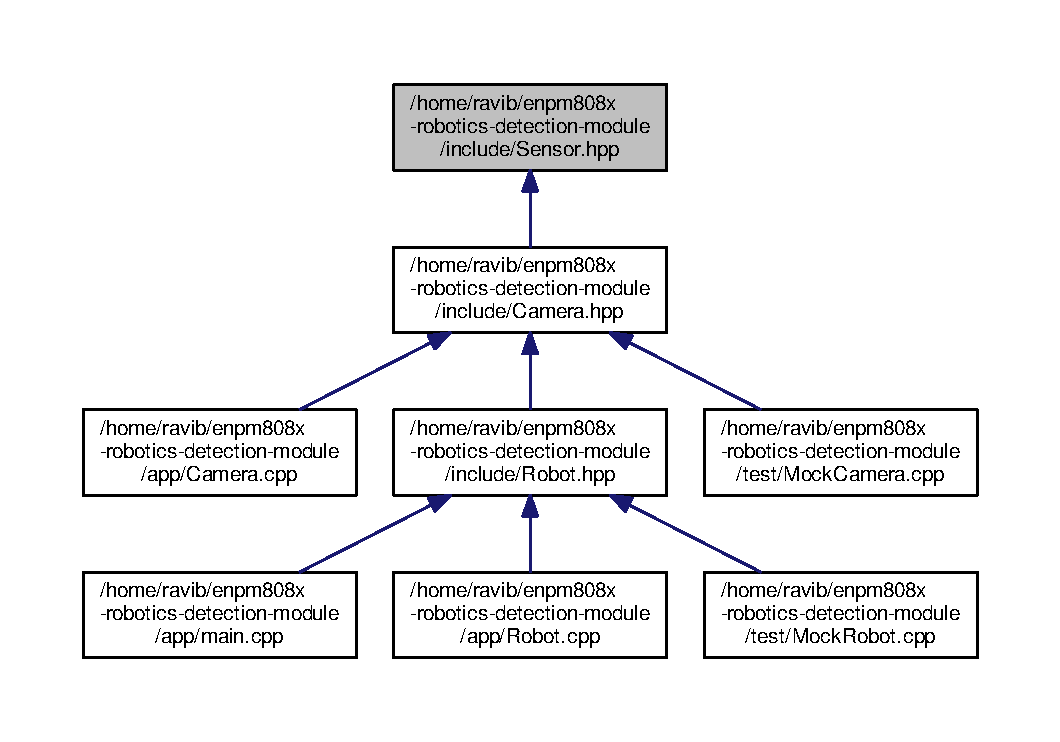
\includegraphics[width=350pt]{_sensor_8hpp__dep__incl}
\end{center}
\end{figure}
\subsection*{Classes}
\begin{DoxyCompactItemize}
\item 
class \hyperlink{class_sensor}{Sensor$<$ T $>$}
\begin{DoxyCompactList}\small\item\em Virtual Class for every sensor. \end{DoxyCompactList}\end{DoxyCompactItemize}

\hypertarget{_l_i_c_e_n_s_e_8md}{}\section{/home/ravib/enpm808x-\/robotics-\/detection-\/module/\+L\+I\+C\+E\+N\+SE.md File Reference}
\label{_l_i_c_e_n_s_e_8md}\index{/home/ravib/enpm808x-\/robotics-\/detection-\/module/\+L\+I\+C\+E\+N\+S\+E.\+md@{/home/ravib/enpm808x-\/robotics-\/detection-\/module/\+L\+I\+C\+E\+N\+S\+E.\+md}}

\hypertarget{readme_8md}{}\section{/home/ravib/enpm808x-\/robotics-\/detection-\/module/readme.md File Reference}
\label{readme_8md}\index{/home/ravib/enpm808x-\/robotics-\/detection-\/module/readme.\+md@{/home/ravib/enpm808x-\/robotics-\/detection-\/module/readme.\+md}}

\hypertarget{_mock_camera_8cpp}{}\section{/home/ravib/enpm808x-\/robotics-\/detection-\/module/test/\+Mock\+Camera.cpp File Reference}
\label{_mock_camera_8cpp}\index{/home/ravib/enpm808x-\/robotics-\/detection-\/module/test/\+Mock\+Camera.\+cpp@{/home/ravib/enpm808x-\/robotics-\/detection-\/module/test/\+Mock\+Camera.\+cpp}}
{\ttfamily \#include $<$gmock/gmock.\+h$>$}\newline
{\ttfamily \#include $<$gtest/gtest.\+h$>$}\newline
{\ttfamily \#include $<$memory$>$}\newline
{\ttfamily \#include \char`\"{}Camera.\+hpp\char`\"{}}\newline
Include dependency graph for Mock\+Camera.\+cpp\+:
\nopagebreak
\begin{figure}[H]
\begin{center}
\leavevmode
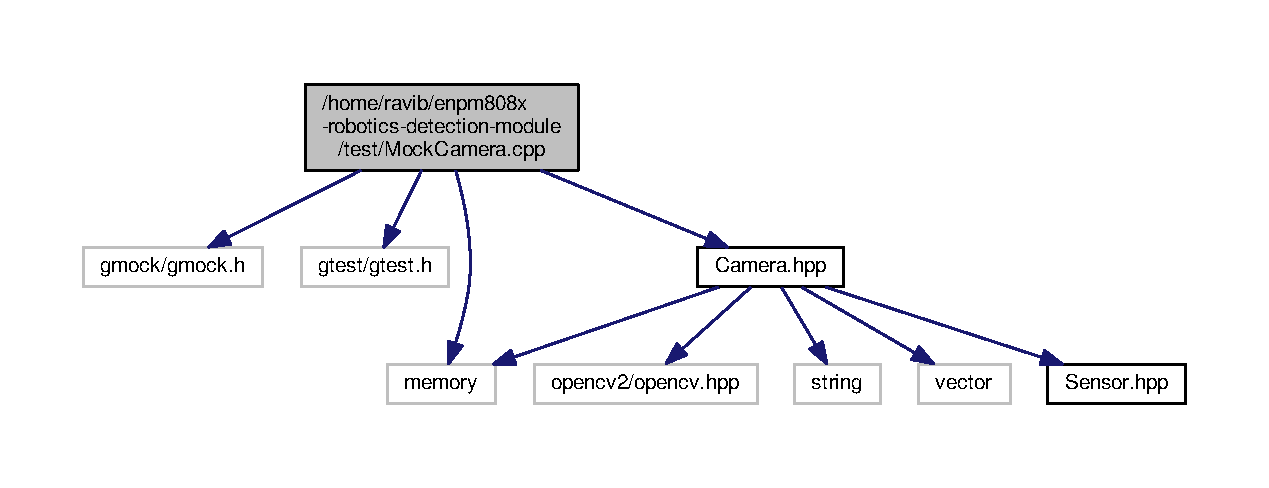
\includegraphics[width=350pt]{_mock_camera_8cpp__incl}
\end{center}
\end{figure}
\subsection*{Functions}
\begin{DoxyCompactItemize}
\item 
\hyperlink{_mock_camera_8cpp_a390a57e39ae9d85d80830b4de977a8fc}{T\+E\+ST} (\hyperlink{class_camera}{Camera}, init)
\item 
\hyperlink{_mock_camera_8cpp_adca5eb672a8fe7c1565267d1043674c1}{T\+E\+ST} (\hyperlink{class_camera}{Camera}, img\+Seq\+\_\+check)
\item 
\hyperlink{_mock_camera_8cpp_a8b910bb6faaaf92c97b81906d74cd055}{T\+E\+ST} (\hyperlink{class_camera}{Camera}, video\+\_\+check)
\end{DoxyCompactItemize}


\subsection{Detailed Description}
\begin{DoxyAuthor}{Author}
Ravi Bhadeshiya 
\end{DoxyAuthor}
\begin{DoxyVersion}{Version}
1.\+0 
\end{DoxyVersion}
\begin{DoxyCopyright}{Copyright}
M\+IT License (c) 2017 Ravi Bhadeshiya 
\end{DoxyCopyright}


\subsection{Function Documentation}
\mbox{\Hypertarget{_mock_camera_8cpp_a390a57e39ae9d85d80830b4de977a8fc}\label{_mock_camera_8cpp_a390a57e39ae9d85d80830b4de977a8fc}} 
\index{Mock\+Camera.\+cpp@{Mock\+Camera.\+cpp}!T\+E\+ST@{T\+E\+ST}}
\index{T\+E\+ST@{T\+E\+ST}!Mock\+Camera.\+cpp@{Mock\+Camera.\+cpp}}
\subsubsection{\texorpdfstring{T\+E\+S\+T()}{TEST()}\hspace{0.1cm}{\footnotesize\ttfamily [1/3]}}
{\footnotesize\ttfamily T\+E\+ST (\begin{DoxyParamCaption}\item[{\hyperlink{class_camera}{Camera}}]{,  }\item[{init}]{ }\end{DoxyParamCaption})}



Definition at line 12 of file Mock\+Camera.\+cpp.

\mbox{\Hypertarget{_mock_camera_8cpp_adca5eb672a8fe7c1565267d1043674c1}\label{_mock_camera_8cpp_adca5eb672a8fe7c1565267d1043674c1}} 
\index{Mock\+Camera.\+cpp@{Mock\+Camera.\+cpp}!T\+E\+ST@{T\+E\+ST}}
\index{T\+E\+ST@{T\+E\+ST}!Mock\+Camera.\+cpp@{Mock\+Camera.\+cpp}}
\subsubsection{\texorpdfstring{T\+E\+S\+T()}{TEST()}\hspace{0.1cm}{\footnotesize\ttfamily [2/3]}}
{\footnotesize\ttfamily T\+E\+ST (\begin{DoxyParamCaption}\item[{\hyperlink{class_camera}{Camera}}]{,  }\item[{img\+Seq\+\_\+check}]{ }\end{DoxyParamCaption})}



Definition at line 18 of file Mock\+Camera.\+cpp.

\mbox{\Hypertarget{_mock_camera_8cpp_a8b910bb6faaaf92c97b81906d74cd055}\label{_mock_camera_8cpp_a8b910bb6faaaf92c97b81906d74cd055}} 
\index{Mock\+Camera.\+cpp@{Mock\+Camera.\+cpp}!T\+E\+ST@{T\+E\+ST}}
\index{T\+E\+ST@{T\+E\+ST}!Mock\+Camera.\+cpp@{Mock\+Camera.\+cpp}}
\subsubsection{\texorpdfstring{T\+E\+S\+T()}{TEST()}\hspace{0.1cm}{\footnotesize\ttfamily [3/3]}}
{\footnotesize\ttfamily T\+E\+ST (\begin{DoxyParamCaption}\item[{\hyperlink{class_camera}{Camera}}]{,  }\item[{video\+\_\+check}]{ }\end{DoxyParamCaption})}



Definition at line 30 of file Mock\+Camera.\+cpp.


\hypertarget{_mock_detection_8cpp}{}\section{/home/ravib/enpm808x-\/robotics-\/detection-\/module/test/\+Mock\+Detection.cpp File Reference}
\label{_mock_detection_8cpp}\index{/home/ravib/enpm808x-\/robotics-\/detection-\/module/test/\+Mock\+Detection.\+cpp@{/home/ravib/enpm808x-\/robotics-\/detection-\/module/test/\+Mock\+Detection.\+cpp}}
{\ttfamily \#include $<$gmock/gmock.\+h$>$}\newline
{\ttfamily \#include $<$gtest/gtest.\+h$>$}\newline
{\ttfamily \#include $<$memory$>$}\newline
{\ttfamily \#include \char`\"{}Detection.\+hpp\char`\"{}}\newline
Include dependency graph for Mock\+Detection.\+cpp\+:
\nopagebreak
\begin{figure}[H]
\begin{center}
\leavevmode
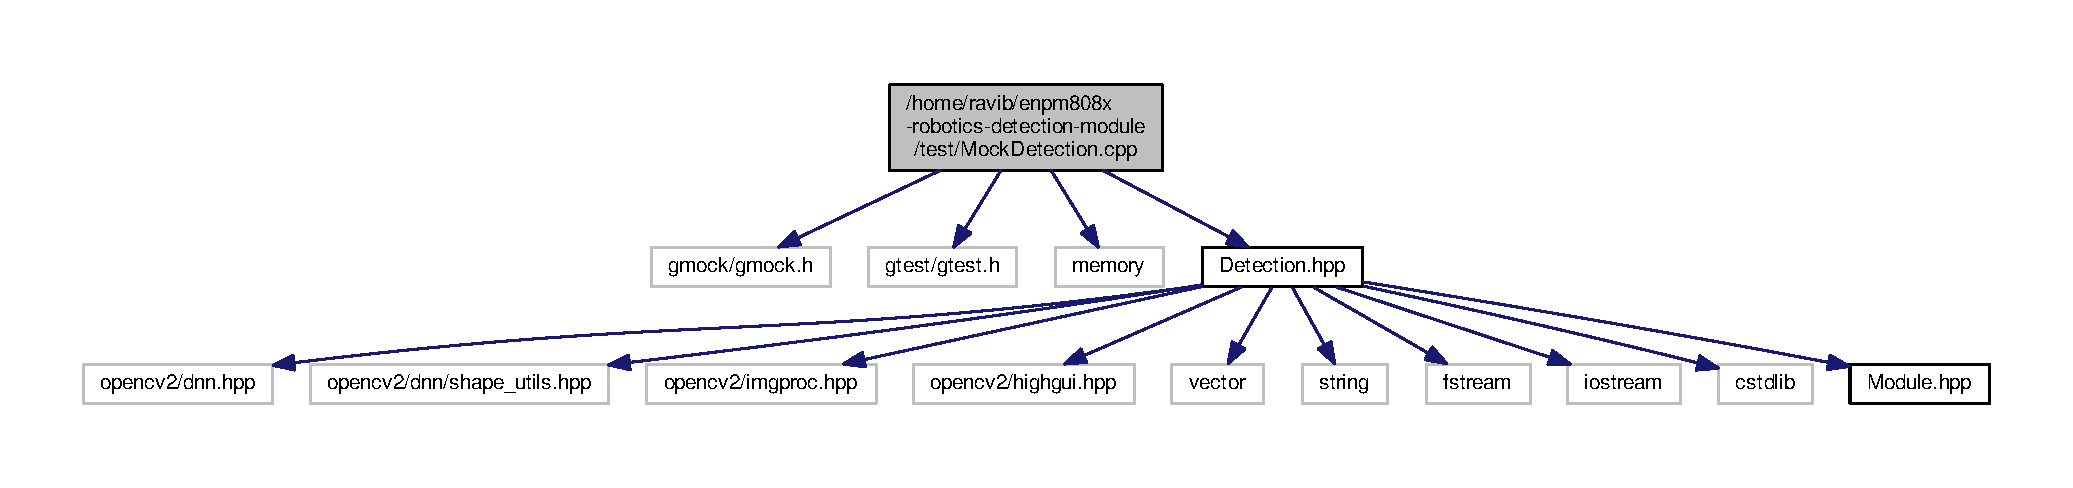
\includegraphics[width=350pt]{_mock_detection_8cpp__incl}
\end{center}
\end{figure}
\subsection*{Functions}
\begin{DoxyCompactItemize}
\item 
\hyperlink{_mock_detection_8cpp_a485d692a7ee42aa99def4eb9285deb10}{T\+E\+ST} (\hyperlink{class_detection}{Detection}, init)
\item 
\hyperlink{_mock_detection_8cpp_a487d465bbfd10bcb4d869e750ed07772}{T\+E\+ST} (\hyperlink{class_detection}{Detection}, detector)
\end{DoxyCompactItemize}


\subsection{Function Documentation}
\mbox{\Hypertarget{_mock_detection_8cpp_a485d692a7ee42aa99def4eb9285deb10}\label{_mock_detection_8cpp_a485d692a7ee42aa99def4eb9285deb10}} 
\index{Mock\+Detection.\+cpp@{Mock\+Detection.\+cpp}!T\+E\+ST@{T\+E\+ST}}
\index{T\+E\+ST@{T\+E\+ST}!Mock\+Detection.\+cpp@{Mock\+Detection.\+cpp}}
\subsubsection{\texorpdfstring{T\+E\+S\+T()}{TEST()}\hspace{0.1cm}{\footnotesize\ttfamily [1/2]}}
{\footnotesize\ttfamily T\+E\+ST (\begin{DoxyParamCaption}\item[{\hyperlink{class_detection}{Detection}}]{,  }\item[{init}]{ }\end{DoxyParamCaption})}



Definition at line 13 of file Mock\+Detection.\+cpp.

\mbox{\Hypertarget{_mock_detection_8cpp_a487d465bbfd10bcb4d869e750ed07772}\label{_mock_detection_8cpp_a487d465bbfd10bcb4d869e750ed07772}} 
\index{Mock\+Detection.\+cpp@{Mock\+Detection.\+cpp}!T\+E\+ST@{T\+E\+ST}}
\index{T\+E\+ST@{T\+E\+ST}!Mock\+Detection.\+cpp@{Mock\+Detection.\+cpp}}
\subsubsection{\texorpdfstring{T\+E\+S\+T()}{TEST()}\hspace{0.1cm}{\footnotesize\ttfamily [2/2]}}
{\footnotesize\ttfamily T\+E\+ST (\begin{DoxyParamCaption}\item[{\hyperlink{class_detection}{Detection}}]{,  }\item[{detector}]{ }\end{DoxyParamCaption})}



Definition at line 23 of file Mock\+Detection.\+cpp.


\hypertarget{_mock_robot_8cpp}{}\section{/home/ravib/enpm808x-\/robotics-\/detection-\/module/test/\+Mock\+Robot.cpp File Reference}
\label{_mock_robot_8cpp}\index{/home/ravib/enpm808x-\/robotics-\/detection-\/module/test/\+Mock\+Robot.\+cpp@{/home/ravib/enpm808x-\/robotics-\/detection-\/module/test/\+Mock\+Robot.\+cpp}}
{\ttfamily \#include $<$gmock/gmock.\+h$>$}\newline
{\ttfamily \#include $<$gtest/gtest.\+h$>$}\newline
{\ttfamily \#include $<$memory$>$}\newline
{\ttfamily \#include \char`\"{}Robot.\+hpp\char`\"{}}\newline
Include dependency graph for Mock\+Robot.\+cpp\+:
\nopagebreak
\begin{figure}[H]
\begin{center}
\leavevmode
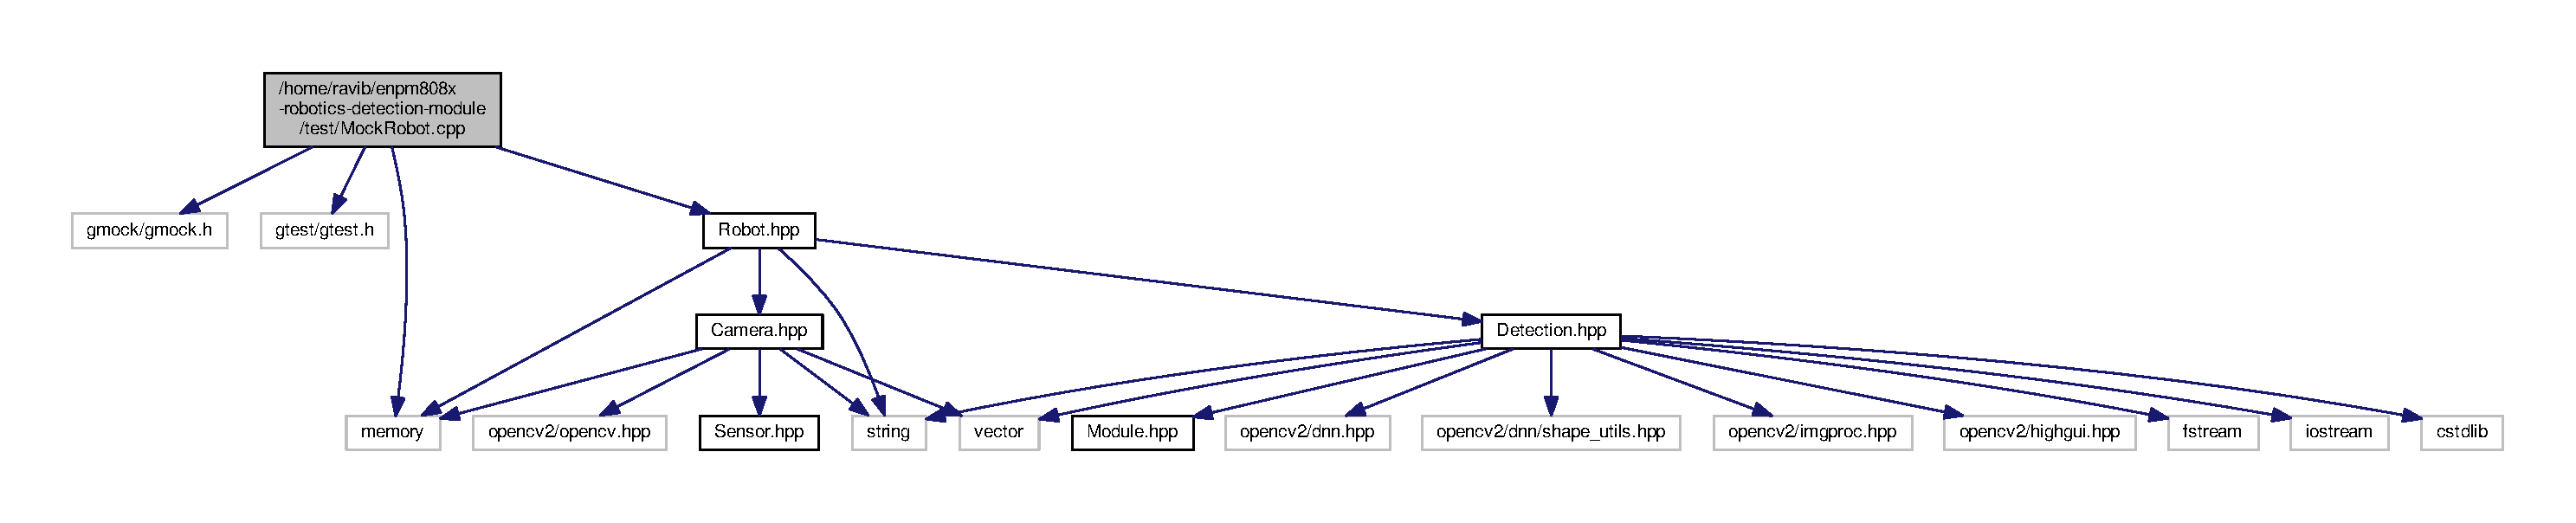
\includegraphics[width=350pt]{_mock_robot_8cpp__incl}
\end{center}
\end{figure}
\subsection*{Functions}
\begin{DoxyCompactItemize}
\item 
\hyperlink{_mock_robot_8cpp_a883145bd6ff7414bf3dfbc96fbe679a0}{T\+E\+ST} (\hyperlink{class_robot}{Robot}, init)
\item 
\hyperlink{_mock_robot_8cpp_a35b0419b4f8f6a38644219cb345540ec}{T\+E\+ST} (\hyperlink{class_robot}{Robot}, setup)
\item 
\hyperlink{_mock_robot_8cpp_a2182e4bd19c25fe494ae42f7dd772842}{T\+E\+ST} (\hyperlink{class_robot}{Robot}, update)
\end{DoxyCompactItemize}


\subsection{Function Documentation}
\mbox{\Hypertarget{_mock_robot_8cpp_a883145bd6ff7414bf3dfbc96fbe679a0}\label{_mock_robot_8cpp_a883145bd6ff7414bf3dfbc96fbe679a0}} 
\index{Mock\+Robot.\+cpp@{Mock\+Robot.\+cpp}!T\+E\+ST@{T\+E\+ST}}
\index{T\+E\+ST@{T\+E\+ST}!Mock\+Robot.\+cpp@{Mock\+Robot.\+cpp}}
\subsubsection{\texorpdfstring{T\+E\+S\+T()}{TEST()}\hspace{0.1cm}{\footnotesize\ttfamily [1/3]}}
{\footnotesize\ttfamily T\+E\+ST (\begin{DoxyParamCaption}\item[{\hyperlink{class_robot}{Robot}}]{,  }\item[{init}]{ }\end{DoxyParamCaption})}



Definition at line 13 of file Mock\+Robot.\+cpp.

\mbox{\Hypertarget{_mock_robot_8cpp_a35b0419b4f8f6a38644219cb345540ec}\label{_mock_robot_8cpp_a35b0419b4f8f6a38644219cb345540ec}} 
\index{Mock\+Robot.\+cpp@{Mock\+Robot.\+cpp}!T\+E\+ST@{T\+E\+ST}}
\index{T\+E\+ST@{T\+E\+ST}!Mock\+Robot.\+cpp@{Mock\+Robot.\+cpp}}
\subsubsection{\texorpdfstring{T\+E\+S\+T()}{TEST()}\hspace{0.1cm}{\footnotesize\ttfamily [2/3]}}
{\footnotesize\ttfamily T\+E\+ST (\begin{DoxyParamCaption}\item[{\hyperlink{class_robot}{Robot}}]{,  }\item[{setup}]{ }\end{DoxyParamCaption})}



Definition at line 18 of file Mock\+Robot.\+cpp.

\mbox{\Hypertarget{_mock_robot_8cpp_a2182e4bd19c25fe494ae42f7dd772842}\label{_mock_robot_8cpp_a2182e4bd19c25fe494ae42f7dd772842}} 
\index{Mock\+Robot.\+cpp@{Mock\+Robot.\+cpp}!T\+E\+ST@{T\+E\+ST}}
\index{T\+E\+ST@{T\+E\+ST}!Mock\+Robot.\+cpp@{Mock\+Robot.\+cpp}}
\subsubsection{\texorpdfstring{T\+E\+S\+T()}{TEST()}\hspace{0.1cm}{\footnotesize\ttfamily [3/3]}}
{\footnotesize\ttfamily T\+E\+ST (\begin{DoxyParamCaption}\item[{\hyperlink{class_robot}{Robot}}]{,  }\item[{update}]{ }\end{DoxyParamCaption})}



Definition at line 26 of file Mock\+Robot.\+cpp.


%--- End generated contents ---

% Bibliography
\newpage
\phantomsection
\bibliographystyle{plain}
\bibliography{}
\addcontentsline{toc}{chapter}{Bibliography}

% Index
\backmatter
\newpage
\phantomsection
\clearemptydoublepage
\addcontentsline{toc}{chapter}{Index}
\printindex

\end{document}
